\documentclass{beamer}
%
% Choose how your presentation looks.
%
\usepackage[T1]{fontenc}
\usepackage[utf8]{inputenc}
\usepackage{lmodern}  
\usepackage{amsmath}
\usepackage{bm}
\usepackage{booktabs}
\usepackage{multirow}
\usepackage{tikz}%boxy  
\usetikzlibrary{calc}
\usepackage{wrapfig}
\usepackage{xcolor}
%
%
%
%
\newcommand*\rbox[1]{\tikz[baseline=(char.base)]{
    \node[shape=rectangle, dashed, draw=red, thick, inner sep=2pt, minimum size=0.6cm] (char) {#1};}}
%
\newcommand{\mytikzmark}[2]{%
  \tikz[remember picture,inner sep=0pt,outer sep=0pt,baseline,anchor=base] 
    \node (#1) {\ensuremath{#2}};}
%
\newcommand*\boxedd[1]{\tikz[baseline=(char.base)]{
    \node[shape=rectangle, dashed, draw=blue, thick, inner sep=2pt, minimum size=0.6cm] (char) {#1};}}
%
%
%
%
% For more themes, color themes and font themes, see:
% http://deic.uab.es/~iblanes/beamer_gallery/index_by_theme.html
%
\mode<presentation>
{
  \usetheme{Darmstadt}      % or try Darmstadt, Madrid, Warsaw, ...
  \usecolortheme{default} % or try albatross, beaver, crane, ...
  \usefonttheme{serif}  % or try default, serif, structurebold, ...
  \setbeamertemplate{navigation symbols}{}
  \setbeamertemplate{caption}[numbered]
  \setbeamertemplate{headline}{}
}
%
%
\title[Block 2]{Block 2 \\  Regression models based on time series\\ Stationarity, cointegration, ECM,\\ Distributed lag models, PAM, AEH}
\author{Advanced Econometrics 4EK608}
\institute{Vysoká škola ekonomická v Praze}
\date{}
%------------------------------------------------------
\begin{document}
 \begin{frame}
  \titlepage
\end{frame}
% Uncomment these lines for an automatically generated outline.
\begin{frame}{Outline}
  \tableofcontents
\end{frame}
%------------------------------------------------------
\section{Time series-based LRMs -- repetition from BSc. courses}
\begin{frame}{Time series-based LRMs -- repetition from BSc. courses}
\begin{itemize}
  \item TS is a stochastic (random) process, a sequence of observations indexed by time. \\Observed TS: one realization of a stochastic process.
  \medskip
  \item Static models
  $$ y_t = \beta_1 + \beta_2 x_t + u_t , \hspace{1cm} t = 1, 2,  \dots, n $$
  \item Finite distributed Lag (FDL) model:
  $$ y_t = \alpha_0 + \beta_0 x_t + \beta_1 x_{t-1} + \beta_2 x_{t-2} + u_t $$
  \item Infinite distributed lag (IDL) model:
  $$ y_t = \alpha_0 + \beta_0 x_t + \beta_1 x_{t-1} + \beta_2 x_{t-2} + \dots + u_t $$
  \item   Dynamic models: lag order\\ For convenience, $\beta$ subscripts follow lag order, \\
  Impact / lagged / long-run multiplier, \\
  Effect of temporary (one-off) $\times$ permanent increase in $x$, \\
  Lag distribution (function).
\end{itemize}
\end{frame}
%------------------------------------------------------
\begin{frame}{G-M assumptions for TSRMs}
\begin{itemize}
\item TS.1 Linearity \\ 
The stochastic process $\{(x_{t1},x_{t2},\dots,x_{tk},y_t);t=1,2,\dots, n \}$ 
follows a linear model $ y_t = \beta_1 + \beta_2 x_{t2} + \dots + \beta_K x_{tK}+u_t$.
\medskip
\item TS.2 No perfect collinearity \\
There is no perfect collinearity among regressors. \\
{\footnotesize Comment: It allows collinearity among regressors.}
\medskip
\item TS.3 Strict exogeneity \\ 
For each $t$, the expected value of error conditionally on the explanatory variables at all time periods is zero: $ E(u_t|\boldsymbol{X})=0, \hspace{0.5cm} t = 1,2,\dots,n$ \\ \medskip
    {\footnotesize Note: Contemporaneous exogeneity (relaxed version): $E(u_t|x_{t1},x_{t2},\dots,x_{tk})=E(u_t|\boldsymbol{x}_t)=0$.}  
\end{itemize}
\end{frame}
%------------------------------------------------------
\begin{frame}{G-M assumptions for TSRMs}
\begin{itemize}
 \item TS.4 Conditional Homoscedasticity 
 $$\textnormal{var}(u_t|\boldsymbol{X})=\textnormal{var}(u_t)=\sigma^2, \hspace{0.5cm} t=1,2,\dots,n$$
 \medskip
 \item TS.5 Serial Correlation (Autocorrelation) is not present $$ \textnormal{corr}(u_t,u_s|\boldsymbol{X}) = 0, \hspace{0.5cm} t\neq s$$
 \medskip
 \item TS.6 Normality \\
 $u_t$ are independent of $\boldsymbol{X}$ and $\textit{i.i.d.}$ :  $u_t \sim N(0,\sigma^2), \textit{i.i.d.} $
  \vspace{0.6cm}
  \item \textbf{CLRM}: Classical linear regression model \\
 TS.1 - TS.6 conditions hold
\end{itemize}
\end{frame}
%------------------------------------------------------
\begin{frame}{Properties of OLS estimators}
\begin{itemize}
\item Under TS.1 - TS.3, OLS estimators are unbiased.
\medskip
\item Under assumptions TS.1 - TS.5, \\ \medskip
$\textnormal{var}(\hat{\beta_j})=\hat{\sigma}^2(\bm{X}^{\prime}\bm{X})^{-1}$~~and~~$\hat{\sigma}^2=\frac{SSR}{n-K-1}$.
\medskip
\item Under assumptions TS.1 - TS.5, \\ \medskip OLS estimators are \textbf{BLUE} (conditional on $\boldsymbol{X}$).
\medskip
\item Under assumptions TS.1 - TS.6, $\hat{\beta}_j$ are normally distributed. Under $H_0$, each $t$ statistics has a $t$ distribution and $F$ statistic has a $F$ distribution (small-sample and asymptotically). The usual construction of confidence intervals is also valid. 
\end{itemize}
\end{frame}
%------------------------------------------------------
\begin{frame}{Trends and spurious regression}
\begin{itemize}
\item Regression: $y$ on $t$ \\ If there is a linear trend in $y$
\vspace{0.5cm}
\item Regression: $\log{y}$ on $t$ \\ Exponential trend, constant rate of growth of $y$
\vspace{0.5cm}
\item Spurious regression: \\ \medskip We can find relationship between two or more trending variables even if it does not exist in reality (non-stationarity and cointegration topics discussed next).
\end{itemize}
\end{frame}
%------------------------------------------------------
\begin{frame}{Detrending and deseasonalizing}
\textbf{Detrending algorithm (based on FWL theorem):}
$$\hat{y_t}=\hat{\beta_1}+\hat{\beta_2}x_{t2}+\hat{\beta_3}x_{t3}+\hat{\beta_4}t$$
\begin{itemize}
\item Regress each variable on constant, time and save residuals $$\ddot{y}_{t}, \ddot{x}_{t2}, \ddot{x}_{t3}, \hspace{0.5cm} t=1,2,\dots, n$$
\item Regress $\ddot{y}_{t}$ on $\ddot{x}_{t2}$, $\ddot{x}_{t3}$
$$\hat{\ddot{y}}_{t}=\hat{\beta_2}\ddot{x}_{t2}+\hat{\beta_3}\ddot{x}_{t3}$$
\item Coefficients $\hat{\beta_2}$, $\hat{\beta_3}$ from this regression are the same as in the original regression 
\end{itemize}
\end{frame}
%------------------------------------------------------
\begin{frame}{Coefficient of determination when $y$ is trending}
\begin{itemize}
\item With trending $y$, coefficient of determination overshoots.
$$\overline{R}^2=1-\frac{\hat{\sigma}^2_u}{\hat{\sigma}^2_y}$$
\begin{itemize}
\item $\hat{\sigma}^2_u$ is unbiased estimator (if trend is among regressors).\\
\medskip
\item With trending $y$, $\hat{\sigma}^2_y=\frac{SST}{(n-1)}$, where $SST=\sum_{t=1}^n (y_t-\overline{y})^2$ is neither unbiased nor consistent estimator.
\end{itemize}
\bigskip
\item Better approach: regress $\ddot{y}_{t}$ on $\ddot{x}_{t1}$, $\ddot{x}_{t2}$.\\ 
\medskip
Coefficient of determination from this regression, i.e.: 
$$R^2=1-\frac{SSR}{\sum^n_{t=1}\ddot{y}^2_t}$$ 
is more reliable (does not overshoot) than that one from the original regression.
\end{itemize}
\end{frame}
%------------------------------------------------------
\begin{frame}{Detrending and deseasonalizing} 
\textbf{Deseasonalizing algorithm (based on FWL theorem):} \\
\footnotesize{Example based on quarterly data} 
$$\hat{y_t}=\hat{\beta_1}+\hat{\beta_2}x_{t2}+\hat{\beta_3}x_{t3}+\hat{\gamma_1}\textit{dummy}1+\hat{\gamma_2}\textit{dummy}2+\hat{\gamma_3}\textit{dummy}3$$
\begin{itemize}
\item Regress variables on constant, seasonal dummies and save residuals: $$\ddot{y}_{t}, \ddot{x}_{t2}, \ddot{x}_{t3}, \hspace{0.5cm} t=1, 2,\dots, n$$
\item Regress $\ddot{y}_{t}$ on $\ddot{x}_{t2}$, $\ddot{x}_{t3}$
$$\hat{\ddot{y}}_{t}=\hat{\beta_2}\ddot{x}_{t2}+\hat{\beta_3}\ddot{x}_{t3}$$
\item Coefficients $\hat{\beta_2}$, $\hat{\beta_3}$ from this regression are the same as in the original regression 
\end{itemize}
\end{frame}
%------------------------------------------------------
\begin{frame}{Stationary and weakly dependent time series}
\begin{itemize}
\item Strict exogeneity, homoscedasticity, absence of serial correlation and normality assumptions are very limiting 
\medskip
\item With large samples, weaker assumptions are sufficient
\medskip
\item For large samples, key assumptions are: \\ \textbf{Covariance stationarity} and \textbf{weak dependency}\\
\medskip
Time series is strictly stationary if its marginal and all joint distributions are invariant across time.
\medskip
\item \textbf{Covariance stationarity:} first two moments and auto-covariance do not change over time.\\
$E(y_t)= \mu,\qquad \textnormal{var}(y_t) = \sigma^2,\qquad \textnormal{cor}(y_t,y_{t+h})=f(h)$
\medskip
\item \textbf{Weak dependency:} correlation between $x_t$ and $x_{t+h}$ ``quickly'' converges to zero with $h$ growing to infinity.
\end{itemize}
\end{frame}
%------------------------------------------------------
\begin{frame}{Stationary and weakly dependent time series}
\begin{itemize}
\item For Central Limit Theorem (CLT) and Law of Large Numbers (LLN) to hold, dependency between observations must not be too strong and must sufficiently quickly decrease with growing time distance between them.
\medskip
\item Time series can be non-stationary and weakly dependent.
\end{itemize}
\begin{block}{Notes on CLT \& LLN}
\textbf{CLT} implies that the sum of independent random variables \\(or weakly dependent RVs) -- if centered and standardized by \\its s.d. -- has an asymptotic distribution $N(0,1)$.\\ \vspace{0.1cm}
\textbf{LLN} theorem implies that the average from a random sample converges in probability to the population average; LLN holds for stationary and weakly dependent series.
\end{block}
\end{frame}
%------------------------------------------------------
\begin{frame}{Stationary and weakly dependent time series}
\textbf{Examples of weakly dependent time series:}
\bigskip
\begin{itemize}
\item Moving average process of order one: \texttt{ma(1)}
$$y_t=e_t+\alpha_1 e_{t-1},$$
where $e_t$ is an $\textit{iid}$ time series.\\ $$\textnormal{corr}(y_t,y_{t+1})=\tfrac{\alpha_1}{1+\alpha_1^2},$$ observations with higher time distance than 1 are uncorrelated.
\bigskip
\item Stable autoregressive process of order 1: \texttt{ar(1)}\\
\medskip
Under stability condition $|\rho|<1$, it can be demonstrated that (Wooldridge, Introductory econometrics, ch. 11.1):
$$y_t=\rho y_{t-1} + e_t \Rightarrow \textnormal{corr}(y_t,y_{t+h})=\rho^h$$
If stability condition holds, TS is weakly dependent because correlation converges  to zero with growing $h$.
\end{itemize}
\end{frame}
%------------------------------------------------------
\begin{frame}{Asymptotic properties of OLS estimators}
\begin{itemize}
\item TS.1' Linearity \\The stochastic process 
$\{(x_{t1},x_{t2},\dots,x_{tk},y_t);t=1,2,\dots, n\}$ follows the linear model $ y_t = \beta_0 + \beta_1 x_{t1} + \dots + \beta_k x_{tk}+u_t$ 
\\ \vspace{0.1cm} We assume both dependent and independent variables are stationary and weakly dependent.
\medskip
\item TS.2' No perfect collinearity \\
There is no perfect collinearity among regressors. \\
{\footnotesize Comment: the same assumption as TS.2}
\medskip
\item TS.3' Contemporaneous exogeneity 
\\Null conditional expected value of errors: 
$$E(u_t|x_{t1},\dots,x_{tk})=E(u_t|\boldsymbol{x}_t)=0$$
\end{itemize}
\end{frame}
%------------------------------------------------------
\begin{frame}{Asymptotic properties of OLS estimators}
\begin{itemize}
\item TS.4' Contemporaneous homoscedasticity
$$\textnormal{var}(u_t|\boldsymbol{x}_t)=\textnormal{var}(u_t)=\sigma^2$$
\vspace{0.5cm}
\item TS.5' No serial correlation \\(autocorrelation in residuals is not present)
$$\textnormal{corr}(u_t,u_s|\boldsymbol{x}_t,\boldsymbol{x}_s ) = 0, t\neq s$$
\end{itemize}
\end{frame}
%------------------------------------------------------
\begin{frame}{Asymptotic properties of OLS estimators}
Under assumptions TS.1', TS.2' and TS.3', \\ \medskip
\begin{itemize}
\item OLS estimators are consistent (not unbiased)\\ 
\medskip
TS.1' - TS.3' $\Rightarrow \textnormal{plim}\,\hat{\beta}_j = \beta_j, \hspace{0.5cm} j=0, 1, \dots, k$
\end{itemize} \bigskip
Removing strict exogeneity (TS.3 $\rightarrow$ TS.3'): no restriction on how $u_t$ is related to regressors in other time periods. Hence: \\
\medskip
\begin{itemize}
\item We allow for feedback from (lagged) explained variable to ``future'' values of explanatory variables 
\medskip
\item We can use lagged dependent variable as regressors.
\end{itemize} \medskip
Theorem: Asymptotic normality of OLS: Under assumptions TS.1' – TS.5', OLS estimators are asymptotically normally distributed. \medskip
\begin{itemize}
\item Usual OLS standard errors, $t$-statistics and $F$-statistics are asymptotically valid.
$$
\hat{\bm{\beta}} \rightarrow N(\bm{\beta}, \hat{\sigma}^2(\bm{X}^{\prime} \bm{X})^{-1} )
\textnormal{~as~} n \rightarrow \infty
$$
\end{itemize}
\end{frame}
%------------------------------------------------------
\begin{frame}{Serial correlation in TSRM}
\begin{itemize}
\item Causes and effects of autocorrelation \\ \bigskip DGP, dynamic (in)completeness of models\\ \medskip unbiased $\hat{\beta}_j$, biased inference
\bigskip
\bigskip
\item FGLS (only with strictly exogenous regressors)
\bigskip
\item OLS + robust inference (Newey-West \& other HAC s.e.)
\end{itemize}
\end{frame}
%------------------------------------------------------
\begin{frame}{Serial correlation in TSRM}
Testing AR(1) with strictly exogenous regressors\\ \medskip
\begin{itemize}
\item $\rho$ estimation:
\begin{align}\nonumber
y_t & = \beta_0+\beta_1 x_{t1}+\dots+\beta_k x_{tk}+u_t \\ \nonumber
u_t & = \rho u_{t-1} + e_t \\ \nonumber
\hat{u}_t &= \rho \hat{u}_{t-1}+error \\ \nonumber
H_0 & : \rho=0 \nonumber
\end{align}
\item Durbin-Watson test: $$d = \frac{\sum \limits^n_{t=2} \big(\hat{u}_t - \hat{u}_{t-1}\big)^2}{\sum \limits^n_{t=1}\hat{u}^2_t}$$.
\begin{itemize}
\item small sample validity (conditions apply)\\
\item $d$-statistic: symmetric distribution $\left\langle 0,4 \right\rangle, \> E(d)=2$
\item $ d \approx 2(1-\hat{\rho}) $    i.e.   $\hat{\rho} \approx 1-d/2$. Test for: \ $ H_0: \rho=0$.
\end{itemize}
\end{itemize}
\end{frame}
%------------------------------------------------------
\begin{frame}{Serial correlation}
Testing serial correlation with general regressors\\ \medskip
\begin{itemize}
\item Testing AR(1):
$$\hat{u}_t=\alpha_0+\alpha_1 x_{t1} + \dots + \alpha_k x_{tk} + \rho \hat{u}_{t-1} + \textit{error}$$
$$H_0 : \rho = 0$$
We can use a heteroscedasticity-robust version of the $t$-test.\\ \bigskip
\item Breusch-Godfrey test for AR($q$) serial correlation:
$$\hat{u}_t=\alpha_0+\alpha_1 x_{t1} + \dots + \alpha_k x_{tk} + \rho_1 \hat{u}_{t-1} +\dots+ \rho_q \hat{u}_{t-q}+\textit{error}  $$
$$H_0 : \rho_1 = \dots = \rho_q = 0$$ \\ \medskip
Use $F$-test \quad or \quad LM-test: $(n-q)R_a^2 \underset{H_0}{\sim} \chi^2_{(q)}$.
\end{itemize}
\end{frame}
%------------------------------------------------------
\begin{frame}{GLSM, matrix form description}
Generalized linear regression model (GLRM) accomodates both autocorrelated and heteroscedastic residuals in the LRM.\\ \medskip
\begin{itemize}
\item GLRM properties:
\begin{itemize}
\item $E(\boldsymbol{u})=\boldsymbol{0}$
\item $E(\boldsymbol{uu}^T)=\sigma^2\boldsymbol{H}$ \\ (i.e. not $\sigma^2 \boldsymbol{I}_{\! n}$) - covariance matrix of disturbances
\end{itemize}
\vspace{0.5cm}
\item Principle of GLSM: \\Transformation of LRM using a transformation matrix $\boldsymbol{T}$ (such that $\bm{THT}^{T}=\bm{I}_n$) to get: \\ \medskip
$\textnormal{var}(\boldsymbol{u}) = \sigma^2 \boldsymbol{I}_{\! n}$ \\ \medskip
in the transformed model.
\end{itemize}
\end{frame}
%------------------------------------------------------
\begin{frame}{GLSM, matrix form description}
\textbf{CLRM:} \hspace{0.2cm} $\boldsymbol{y}=\boldsymbol{X}\boldsymbol{\beta}+\boldsymbol{u}$; OLS estimator: $\boldsymbol{\hat{\beta}}=(\boldsymbol{X}^T\boldsymbol{X})^{-1}\boldsymbol{X}^T\boldsymbol{y}$ \\
~\\
\textbf{GLRM} transformation principle:  $\boldsymbol{T}\boldsymbol{y}=\boldsymbol{TX}\boldsymbol{\beta}+\boldsymbol{T}\boldsymbol{u}$\\ \medskip
\begin{itemize}
\item For covariance matrix of the transformed model, we get:
$$E(\boldsymbol{T}\boldsymbol{u}(\boldsymbol{T}\boldsymbol{u})^T)=
E(\boldsymbol{T}\boldsymbol{u}\boldsymbol{u}^T\boldsymbol{T}^T)=\boldsymbol{T} E(\boldsymbol{u}\boldsymbol{u}^T)\boldsymbol{T}^T=\sigma^2\boldsymbol{THT}^T$$
We need $\boldsymbol{THT}^T \! = \boldsymbol{I}$; from this relation we derive the transformation matrix $\boldsymbol{T}$.
Transformation gives us model that fulfills previously broken G-M assumption.
\end{itemize}
\end{frame}
%------------------------------------------------------
\begin{frame}{GLSM, matrix form description}
\textbf{GLSM algorithm:} \\ \medskip
\begin{enumerate}
\item Estimate the model using OLS.
\item Test assumption $E(\boldsymbol{uu}^T)=\sigma^2 \boldsymbol{I}_n$, if  broken:
\item Find/set appropriate transformation matrix $\boldsymbol{T}$.
\item Multiply variables of the model by $\boldsymbol{T}$, to get transformed variables.
\item Estimate the model with transformed variables (use OLS for estimation).
\item If necessary, reverse-transform the model estimated to get parameter estimates for the original specification of the LRM.
\end{enumerate}
\end{frame}
%------------------------------------------------------
\begin{frame}{GLSM, matrix form description}
\begin{itemize}
\item Matrices $\boldsymbol{H}$ and $\boldsymbol{T}$ of the GLSM algorithm differ for heteroscedasticity  and autocorrelation.
\vspace{0.2cm}
\begin{itemize}
\item heteroscedasticity (CS data, matrix form, quick recap):\\
$$\sigma^2 \bm{H} = \sigma^2 
\begin{bmatrix}
    h_1&  0 & \cdots & 0\\
    0 &  h_2&  \cdots & 0\\ 
     &    &  \vdots& \\ 
     0 & 0 & \cdots & h_n 
\end{bmatrix} = 
\begin{bmatrix}
    \sigma^2_1&  0 & \cdots & 0\\
    0 &  \sigma^2_2&  \cdots & 0\\ 
     &    &  \vdots& \\ 
     0 & 0 & \cdots & \sigma^2_n 
\end{bmatrix}
$$
GLS: $\bm{\hat{\beta}}=(\bm{X}^T \bm{\hat{H}}^{-1} \bm{X})^{-1} \bm{X}^T \bm{\hat{H}}^{-1} \bm{y}$\\
where WLS or FGLS method is used to estimate/set $\bm{\hat{H}}$.
\end{itemize}
\end{itemize}
\end{frame}
%------------------------------------------------------
\begin{frame}{GLSM, matrix form description}
Autocorrelation (matrix form):
\begin{itemize}
\item Let's assume autocorrelation of the AR(1) form $u_t = \rho u_{t-1}+ \varepsilon_t$  ; \\ where $\rho$ is coefficient of autocorrelation $\rho \in (-1; 1)$
\end{itemize}
\vspace{0.2cm}
If we know the autocorrelation coefficient $\rho$,  matrix $E(\boldsymbol{uu}^T)$ is :
$$E(\boldsymbol{uu}^T)= \sigma^2_u\bm{H} = \frac{\sigma^2_{\varepsilon}}{1-\rho^2}
    \begin{bmatrix}
    1&  \rho & \rho^2 & \rho^3 & \cdots & \rho^{n-1}\\
    \rho &  1&  \rho & \rho^2 & \cdots & \rho^{n-2} \\ 
    \rho^2 &  \rho &  1& \rho  & \cdots & \rho^{n-3} \\ 
    \cdots & \cdots & \cdots & \cdots & \cdots & \cdots \\
     \rho^{n-1} & \rho^{n-2} & \rho^{n-3} & \cdots & \rho & 1
\end{bmatrix}$$
( we assume homoscedasticity and known variance $\textnormal{var}(u_t)$ )
\end{frame}
%------------------------------------------------------
\begin{frame}{GLSM, matrix form description}
\begin{itemize}
\item Explanation of matrix $E(\boldsymbol{uu}^T)$: start with $u_t = \rho u_{t-1}+ \varepsilon_t$\\
$u_t= \varepsilon_t + \rho \varepsilon_{t-1} + \rho^2 \varepsilon_{t-2} + \dots$ \qquad where $\varepsilon$ are $i.i.d.$\\
Hence, $\sigma^2_u \equiv \textnormal{var}(u_t)= 
\sigma^2_{\varepsilon} + \rho^2 \sigma^2_{\varepsilon} + \rho^4 \sigma^2_{\varepsilon} 
+ \rho^6 \sigma^2_{\varepsilon} + \dots
= \frac{\sigma^2_{\varepsilon}}{1-\rho^2}$\\
(Note: $\textnormal{cov}(u_t,u_{t+s})=\rho^s \sigma^2_u$ is independent of $t$ if $|\rho|<1$.)\\
\vspace{0.3cm}
\item That is why: 
$H=\begin{bmatrix}
    1&  \rho & \rho^2 & \rho^3 & \cdots & \rho^{n-1}\\
    \rho &  1&  \rho & \rho^2 & \cdots & \rho^{n-2} \\ 
    \rho^2 &  \rho &  1& \rho  & \cdots & \rho^{n-3} \\ 
    \cdots & \cdots & \cdots & \cdots & \cdots & \cdots \\
     \rho^{n-1} & \rho^{n-2} & \rho^{n-3} & \cdots & \rho & 1
\end{bmatrix}$
\vspace{0.3cm}
\item Usually, we do not know the matrix $\boldsymbol{H}$, it must be estimated. In such case, we call the method Feasible General Least Squares (FGLS).
\end{itemize}
\end{frame}
%------------------------------------------------------
\begin{frame}{GLSM, matrix form description}
\textbf{Prais -- Winsten method (transformation)}
\begin{itemize}
\item Transformation by $\boldsymbol{T}$: transformed vector $\boldsymbol{y}$ and matrix $\boldsymbol{X}$
$$\boldsymbol{T}=\sqrt[]{\frac{1}{1-\rho^2}}
\begin{bmatrix}
 \sqrt[]{1-\rho^2}&  0 & 0 & 0\\
 - \rho &  1&  0 & 0\\ 
 \cdots & \cdots & \cdots & \cdots \\
0 &  -\rho &  1& 0\\ 
0 & 0 & -\rho &1 
\end{bmatrix}, \,\,
\boldsymbol{y^\ast}=
\begin{bmatrix}
y_1\sqrt[]{1-\rho^2}\\
y_2-\rho y_1\\
y_3-\rho y_2 \\
\cdots
\end{bmatrix},
$$ $$
\boldsymbol{X^\ast}=\begin{bmatrix}
\sqrt[]{1-\rho^2} & x_{11}\sqrt[]{1-\rho^2} & x_{21}\sqrt[]{1-\rho^2}\\
1-\rho & x_{12}-\rho x_{11} & x_{22}-\rho x_{21} \\
1-\rho & x_{13}-\rho x_{12} & x_{23}-\rho x_{22} \\
\cdots & \cdots & \cdots &
\end{bmatrix}
$$
\item P-W  transformation: quasi-differencing of all variables of the LRM and an approximation for the first period. In the transformation, we skip the fraction in front of $\boldsymbol{T}$-matrix. As a constant, it does not influence the regression result.
\end{itemize}
\end{frame}
%------------------------------------------------------
\begin{frame}{GLSM, matrix form description}
\textbf{Cochrane-Orcutt method (transformation)}
\begin{itemize}
\item P-W method without the approximation of the first observation.
\end{itemize}
\vspace{1cm}
For both the P-W and C-O methods, we usually use iterations to make the estimates of the autoregressive coefficient and regression parameters of the model more accurate.
\end{frame}
%------------------------------------------------------
\section{Stationarity, unit root tests, cointegration}
\begin{frame}{Stationarity, unit root tests, cointegration}
  \begin{itemize}
      \item Stationarity
      \bigskip
      \item Unit root tests
      \bigskip
      \item Cointegration
  \end{itemize}  
\end{frame}
%------------------------------------------------------
\begin{frame}{Weakly and strongly dependent TS}
Weakly dependent time series
  \vspace{0.4cm}
\begin{itemize}
  \item Moving average process of order one \texttt{ma(1)} $x_t=e_t+\alpha_1 e_{t-1}$, where $e_t$ is $\textit{i.i.d.}$ time series. \\Observations with higher time distance than 1 are uncorrelated. This process is stationary.
  \vspace{0.7cm}
  \item For stable autoregressive process of order 1 \texttt{ar(1)}: \\ \smallskip
  $y_t = \rho_1 y_{t-1} + e_t \Rightarrow \textnormal{cor}(y_t,y_{t+h})=\rho^h_1$\\
  \vspace{0.4cm}
  If stability condition $|\rho|<1$  holds, the process is weakly dependent because correlation converges to zero with growing $h$. Also, this process is stationary for $y_0 =0$.
  \vspace{0.4cm}
\end{itemize}
\end{frame}
%---------------------------------------------
\begin{frame}{Weakly and strongly dependent TS}
Strongly dependent time series:\\
Random walk:  
\begin{align}\nonumber
y_t &= y_{t-1}+e_t \\\nonumber 
y_t &= y_{t-2}+e_{t-1}+e_t \\\nonumber
y_t &= y_{t-3}+e_{t-2}+e_{t-1}+e_t \\\nonumber
& \cdots \\ \nonumber
y_t &= y_0 + e_1 + \dots +e_{t-1} + e_t
\end{align} 
Shocks have permanent effects, the series is not covariance stationary and is strongly dependent.
\begin{align}\nonumber
E(y_t) & =E(y_0) \\\nonumber
\textnormal{var}(y_t) & =\sigma^2_e t \\\nonumber
\textnormal{cor}(y_t,y_{t+h}) & =\sqrt[]{t/(t+h)}
\end{align} 
Correlation decreases very slowly and speed depends on $t$.
\end{frame}
%---------------------------------------------
\begin{frame}{Strongly dependent TS}
\begin{itemize}
\item Two realizations of a random walk \\
\vspace{0.5cm}
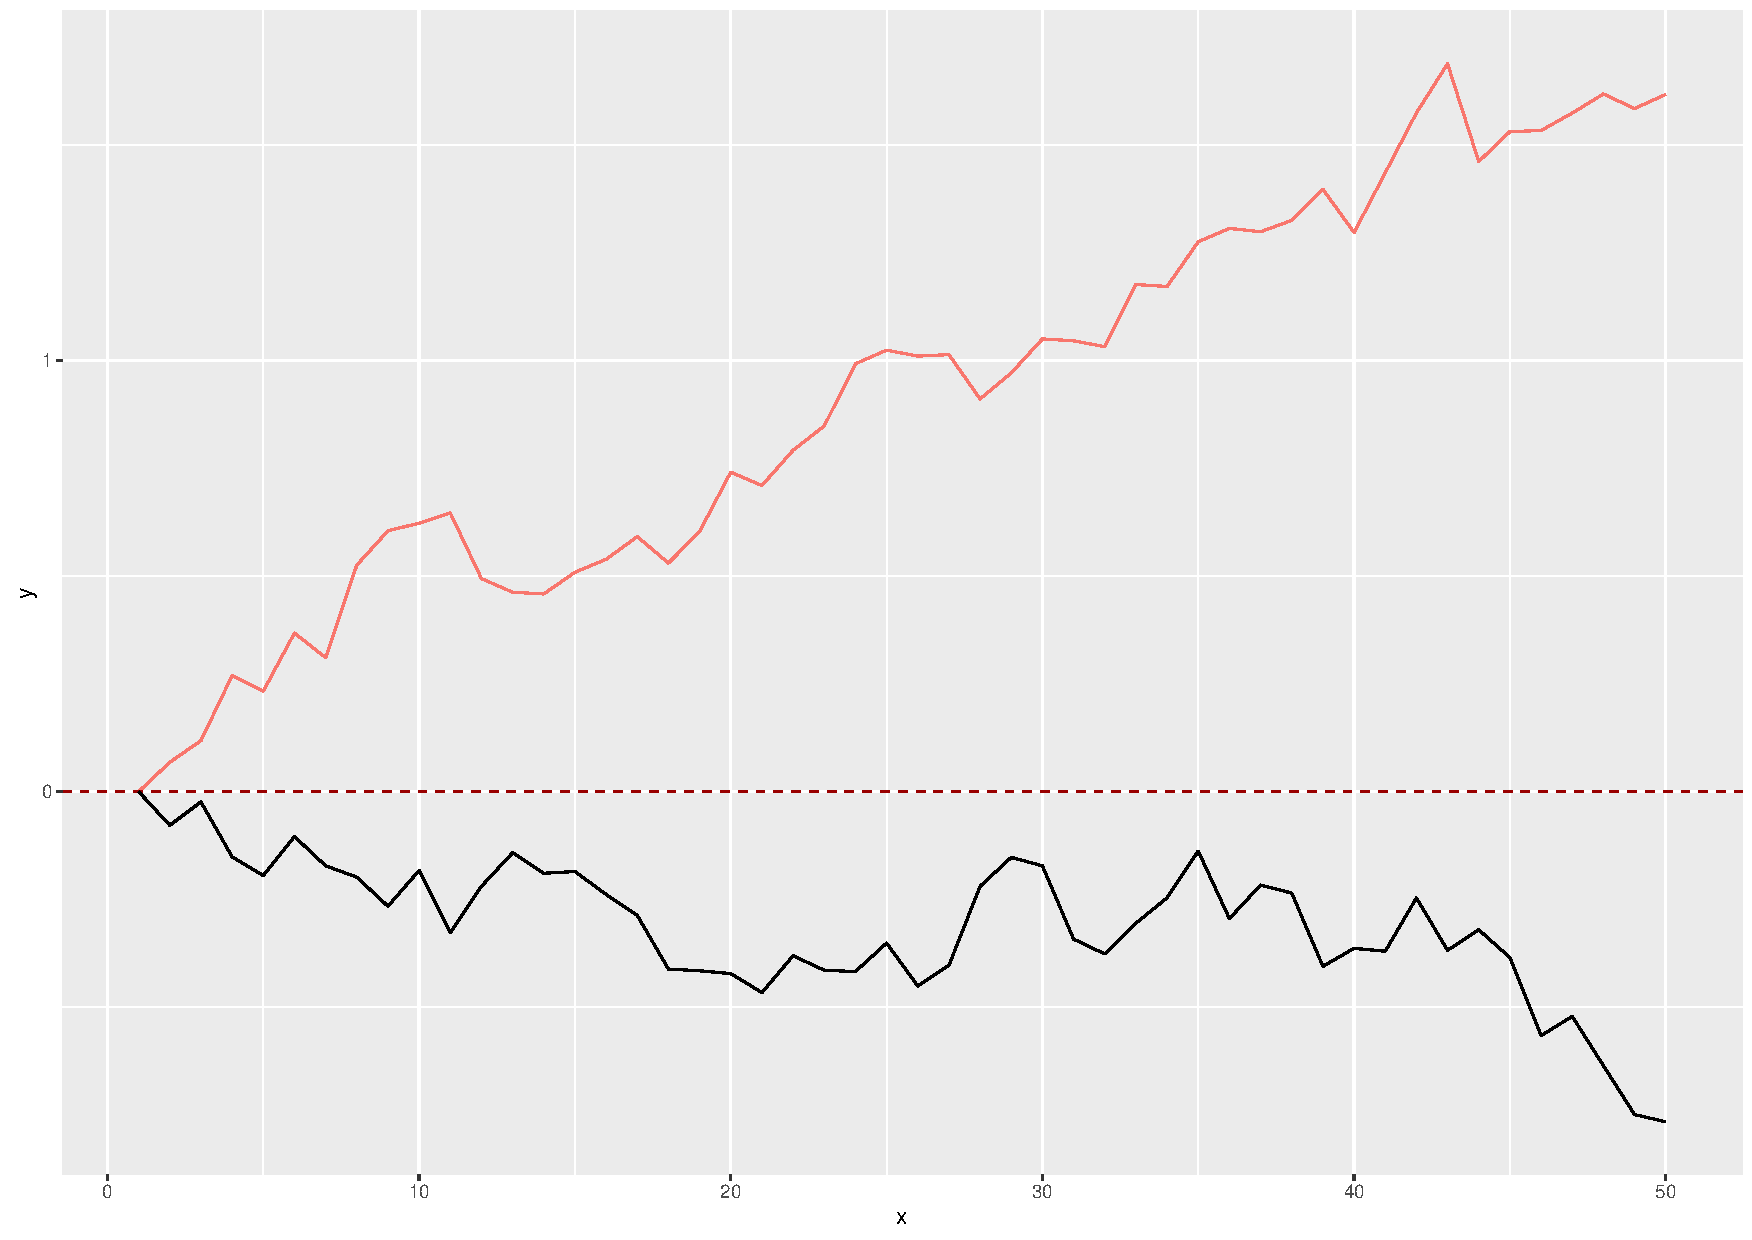
\includegraphics[width=0.7\textwidth]{img/random_walk.pdf}
\end{itemize}
\end{frame}
%---------------------------------------------
\begin{frame}{Strongly dependent TS}
\begin{itemize}
\item Random walk with a drift
$$ y_t=\alpha_0+y_{t-1}+e_t \Rightarrow y_t =\alpha_0 t + e_{t} + e_{t-1} +  \dots +e_1 + y_0$$
A linear trend with random walk around the trend. \\ It is neither covariance stationary nor weakly dependent.
\begin{align}\nonumber
E(y_t) & =\alpha_0 t +E(y_0)\\\nonumber
\textnormal{var}(y_t) & =\sigma^2_e t\\\nonumber
\textnormal{cor}(y_t,y_{t+h}) & =\sqrt[]{t/(t+h)}
\end{align} 
Correlation decreases very slowly and decline speed depends on $t$.
\end{itemize}
\end{frame}
%---------------------------------------------
\begin{frame}{Weakly and strongly dependent TS}
\begin{itemize}
\item Realization of random walk with a drift \\ 
\vspace{0.2cm}
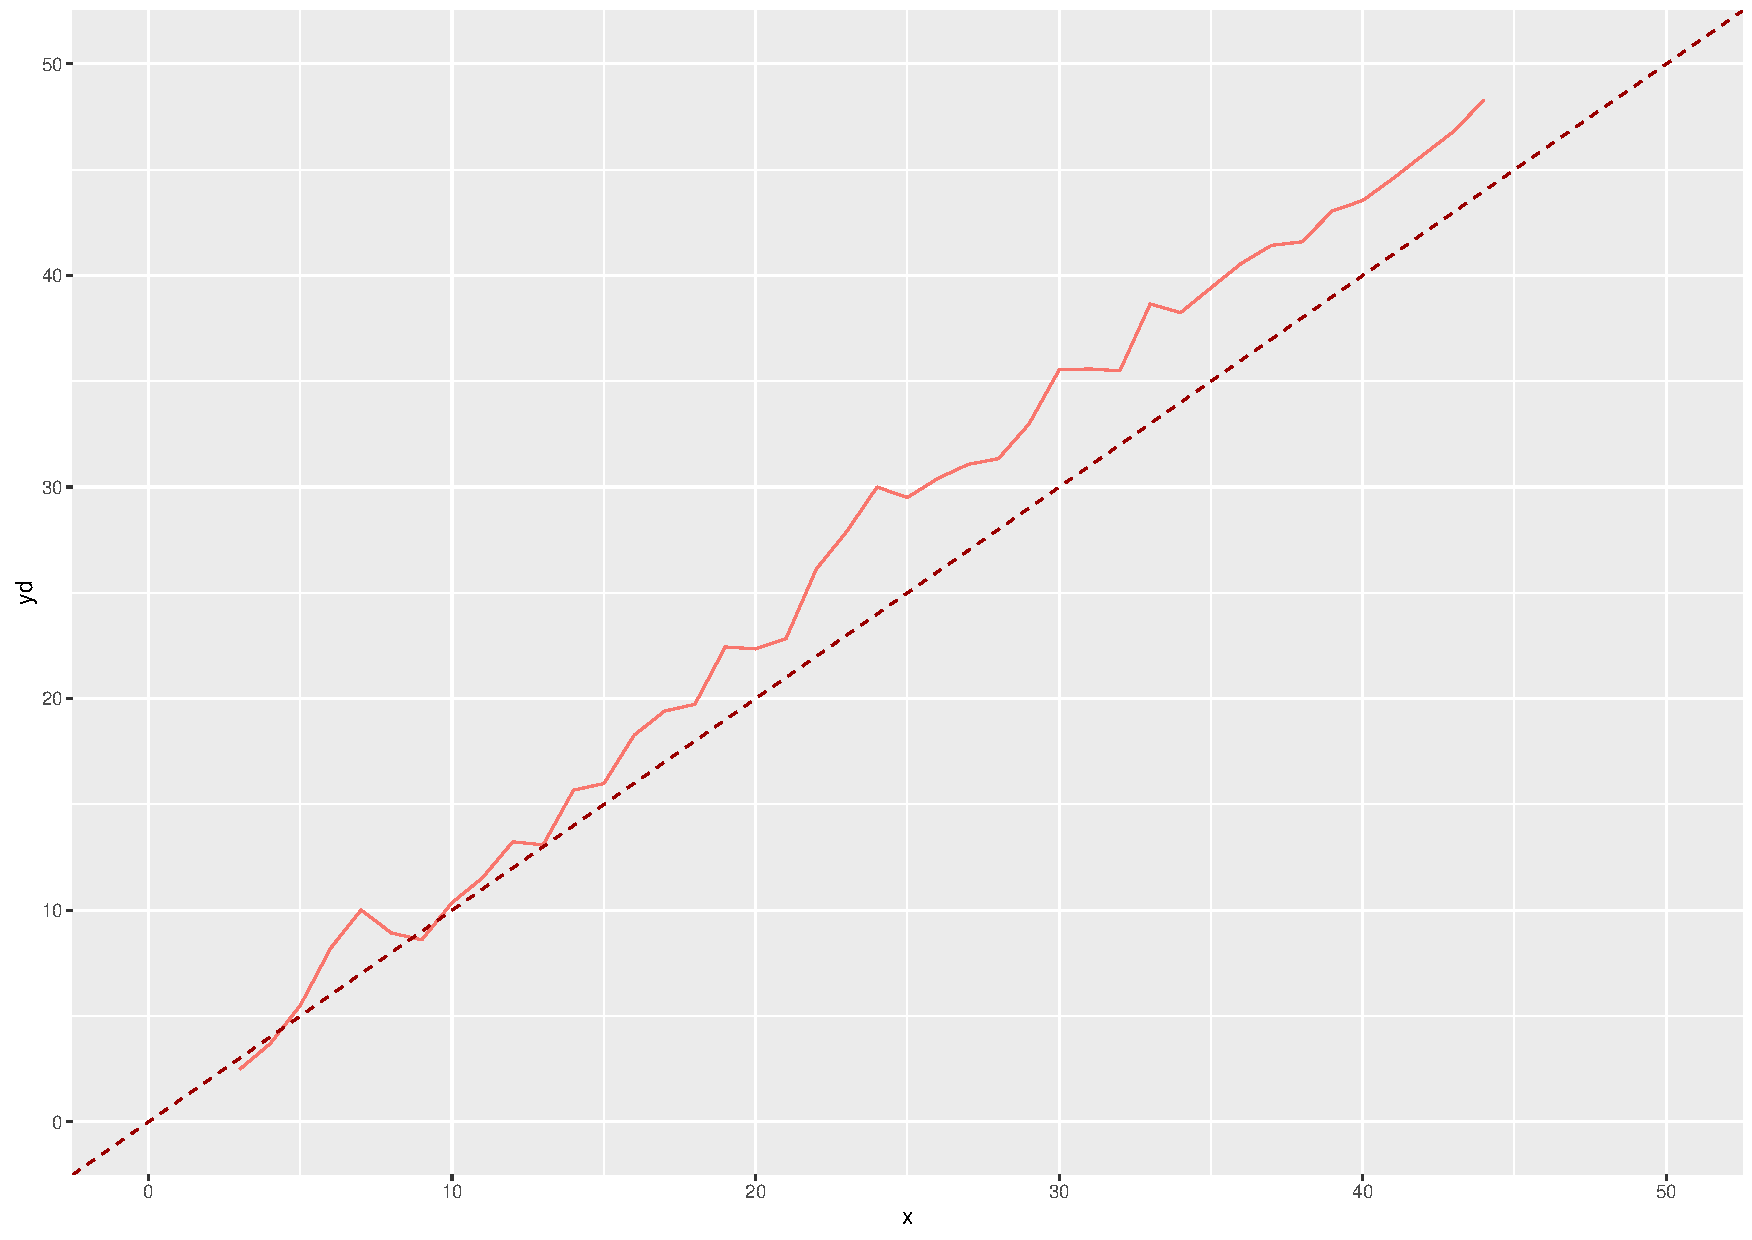
\includegraphics[width=0.7\textwidth]{img/random_walk_drift.pdf}
\item Different realizations of trending TS (weakly dependent around the trend) may produce similar time series.
\end{itemize}
\end{frame}
%---------------------------------------------
\subsection{Unit root tests}
\begin{frame}{Weakly and strongly dependent TS}
$y_t = \boxedd{$1 \cdot y_{t-1}$} + \boxedd{$u_t$} = y_{t-1} + u_t$
\medskip
\begin{itemize}
\item Unit root process: $y_t = y_{t-1} + u_t$; \quad  \\
where: $u_t$ is a weakly dependent series.
\item Random walk is a special case of the unit root process \\where: $u_t \sim \textit{Distr} \, (0, \sigma_u^2), \textit{iid}$
\bigskip
\end{itemize}
We need to distinguish strongly and weakly dependent TS:
%\vspace{0.5cm}
\begin{itemize}
\item Economic reasons: \\ In strongly dependent series, shocks or policy changes  have  long or permanent effects; in weakly dependent series, their effect  is only temporary.
\item Statistical reasons: \\ Analysis with strongly dependent series must be handled in specific ways.
\end{itemize}
\end{frame}
%---------------------------------------------
\begin{frame}{Integrated series}
\textbf{Terminology - Order of integration }
\vspace{0.5cm}
\begin{itemize}
\item Weakly dependent TS are integrated of order zero: $I(0)$.
\vspace{0.2cm}
\item If we have to difference a TS once to get a weakly dependent TS, then it is integrated of order 1: $I(1)$.
\vspace{0.2cm}
\item Example of a $I(1)$ process:
\begin{align}\nonumber
y_t & =y_{t-1}+e_t  \hspace{0.55cm} \Rightarrow \Delta y_t = y_t-y_{t-1}=e_t \\\nonumber
 \log{y_t} & =\log{y_{t-1}}+e_t  \Rightarrow \Delta \log{y_t}=e_t
 \end{align} 
 \item A time series is integrated of order $d$: $I(d)$, if it becomes \\a weakly dependent TS after being differenced $d$ times.
\end{itemize}
\end{frame}
%---------------------------------------------
\begin{frame}{Unit roots tests}
Unit root tests help to decide if a time series is $I(0)$ or not
\vspace{0.4cm}
\begin{itemize}
\item Use either some informal procedure or a unit root test
\vspace{0.4cm}
\item Informal procedures
\begin{itemize}
\item Analyze autocorrelation of the first order
$$\hat{\rho}_1=\hat{\textnormal{corr}}(y_t,y_{t-1})$$
\item If $\hat{\rho}_1$ approaches 1, it indicates that the series can have unit root. Alternatively, it could have a deterministic trend.
\end{itemize}
\item We can analyze sample autocorrelations using \\a correlogram
\end{itemize}
\end{frame}
%---------------------------------------------
\begin{frame}{Unit root tests}
Correlogram:  
$\, \, \, \, \rho_h = \frac{\textit{cov} \, (y_t, y_{t-h})}{\sigma_{y_t} \cdot \sigma_{y_{t-h}}}$
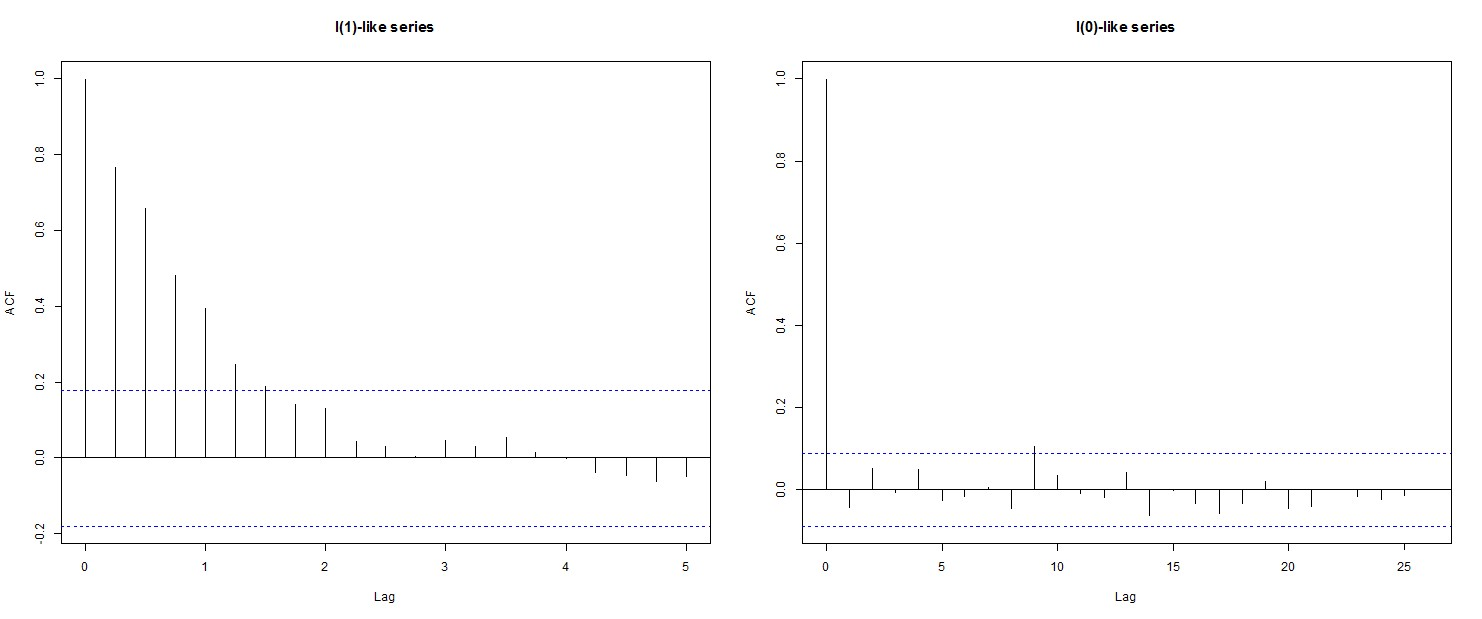
\includegraphics[width=1\textwidth]{img/corelogramWeek2.jpg}
\hspace{1.5cm} $I(1)$-like series \hspace{3 cm} $I(0)$-like series
\end{frame}
%---------------------------------------------
\begin{frame}{Unit root tests}
\textbf{Dickey-Fuller (DF) test} – motivation \\
\medskip
Unit root test in an \texttt{ar(1)} process: \\
\medskip
$y_t = \alpha + \rho y_{t-1} + e_t$\\
\medskip
$ H_0 : \rho = 1, \> \> \> H_1 : \rho <1$ \\
\medskip
\begin{itemize}
\item Under $H_0$, $y_t$ has a unit root. 
\begin{itemize}
\item[$\circ$] For  $\rho =1 \ \wedge \ \alpha =0 \rightarrow y_t$     is a random walk.
\item[$\circ$] For  $\rho =1 \ \wedge \ \alpha \neq 0 \rightarrow y_t$     is a randomw walk with a drift   \\and $E(y_t)$ is a linear function of $t$ .
\end{itemize}
\item Under $H_1$, $y_t$  is a weakly dependent \texttt{ar(1)} process. \\
\bigskip
\end{itemize}
\medskip
\end{frame}
%---------------------------------------------
\begin{frame}{Unit root tests}
\textbf{Dickey-Fuller (DF) test} – motivation \\
\medskip
Unit root test in an \texttt{ar(1)} process: \\
\medskip
$y_t = \alpha + \rho y_{t-1} + e_t$\\
\medskip
$ H_0 : \rho = 1, \> \> \> H_1 : \rho <1$ \\
\medskip
For DF tests, $H_1 : \rho <1$ is a common simplification to the full space of alternatives to $H_0: \rho = 1$.
\begin{itemize}
\item For $|\rho|<1$, $\,\, y_t$  is weakly dependent (as $\textit{plim} \> \rho^h=0$)\\
However, if unit root is likely to be present, the probability of $\rho<0$ is negligible.
\item We usually ignore the possibility of $\rho >1$   , as it would lead to explosive behavior in $y_t$. \\
\dots $|\rho|>1$ would allow for explosive oscillations in $y_t$.
\end{itemize}
\end{frame}
%---------------------------------------------
\begin{frame}{Dickey Fuller (DF) test}
\small
\begin{itemize}
\item Basic equation for unit root test in an \texttt{ar(1)} process: \qquad $ y_t = \alpha + \rho y_{t-1} + e_t $ \\
\item For DF test, we apply a suitable transformation to $y_t$:  \\we subtract $y_{t-1}$ from both sides of the equation:
\begin{flalign*}
& \Delta y_t  = \alpha + (\rho - 1) y_{t-1} + e_t; \text{ apply substitution: } \theta=(\rho-1)&&\\
& \text{i.e.} && \\
& \Delta y_t  = \alpha + \theta y_{t-1} + e_t;  \textrm{ now:} 
\end{flalign*}
\item We use a $t$-ratio for testing $H_0:\theta = 0. $   However:\\
Under $H_0$, $t$-ratios don't have a $t$-distribution, but follow a $DF$-distribution.  (-negative- critical values of the $DF$ distribution are much farther from zero)
\item Critical values for the $DF$ distribution are available from statistical tables and implemented in most relevant SW packages.
\end{itemize}
\begin{tikzpicture}[<-,overlay,remember picture,inner sep=1.5pt,shorten <=0.2em,font=\small]
\tikzset{
    mynode/.style={rectangle, minimum size=3cm, text width=6cm}
}
\node[mynode] at (9,4.2)(box){$H_0 \  : \rho = 1 \Leftrightarrow H_0 : \theta = 0$ \\
$H_1 \ : \rho < 1 \Leftrightarrow H_1 : \theta < 0$};
\tikzset{
    mynode/.style={rectangle, dashed, very thick, draw=red, minimum size=0.9cm, text width=1.6cm}
}
\node[mynode] at (9,4.2) (A){};
\end{tikzpicture}
\end{frame}
%---------------------------------------------
\begin{frame}{DF test \& ADF test}
\footnotesize
Unit root time series can manifest various levels of complexity. Hence, DF  test is usually performed using the following three specifications: \\
\begin{minipage}[c]{.1\textwidth}
\begin{flalign*}
\Delta y_t  = \quad  & \theta y_{t-1} + e_t &&  \\
\Delta y_t  = \alpha \ + \ & \theta y_{t-1} + e_t && \\
\Delta y_t  = \alpha \ + \ & \theta y_{t-1} + \delta t + e_t && \\
\end{flalign*}
\end{minipage}
%
\begin{minipage}[c]{.5\textwidth}
random walk \\
random walk with a drift\\
random walk with a drift and trend
\end{minipage}
% 
\\
DF test is the same ($H_0: \theta = 0$) for all specifications   /critical values difffer/ \\
\medskip
\underline{Augmented Dickey-Fuller (ADF) test} is a common generalization of DF test\\
(example: Augmentation of the DF test for the $2^{nd}$ specification) 
$$\Delta y_t = \alpha + \rbox{$\theta y_{t-1}$} + \gamma_1 \Delta y_{t-1} + \dots + \gamma_p \Delta y_{t-p} + e_t$$
\begin{itemize}
\item When estimating $\theta$, we control for possible $\textit{ar}(p)$ behavior in $\Delta y_t$. 
\item ADF test has the same null hypothesis as a DF test $\rightarrow$ $H_0: \theta = 0$.
\end{itemize}
\begin{tikzpicture}[<-,overlay,remember picture,inner sep=1.5pt,shorten <=0.2em,font=\small]
\tikzset{
     mynode/.style={rectangle, dashed, very thick, draw=red, minimum height=1.5cm, text width=0.8cm}
}
\node[mynode] at (2,5.5)(box){};
\end{tikzpicture}
\end{frame}
%---------------------------------------------
\begin{frame}{Unit root tests in R: package \{urca\}}
Description of the options for the \texttt{ur.df()} function:
\medskip
\begin{enumerate}
\item \texttt{type "none"} \\
$\Delta y_t = \theta y_{t-1} + e_t$ ~\\
\texttt{tau1:} we test for $H_0: \theta = 0$ (unit root) 
\medskip
\item \texttt{type "drift"} \\
$\Delta y_t = \alpha + \theta y_{t-1} + e_t$ ~\\
\texttt{tau2:} $H_0: \theta = 0$ (unit root) \\
\texttt{phi1:} $H_0: \theta = \alpha = 0$ (unit root and no drift) 
\medskip
\item \texttt{type "trend"} \\
$\Delta y_t = \alpha + \theta y_{t-1} + \delta t + e_t$ ~\\
\texttt{tau3:} $H_0: \theta = 0$ (unit root) \\
\texttt{phi2:} $H_0: \theta = \alpha = \delta = 0$ (unit root, no drift, no trend) 
\texttt{phi3:} $H_0: \theta = \delta = 0$ (unit root and no trend) 
\end{enumerate}
Multiple other unit root tests exist: \\(KPSS, tests for seasonal data, break in the DGP, etc.).
\end{frame}
%---------------------------------------------
\begin{frame}{Unit root tests}
\begin{itemize}
\item ADF test for TS with trend
$$ \Delta y_t = \alpha  + \theta y_{t-1} + \delta t + \gamma_1\Delta y_{t-1}+\dots+\gamma_p\Delta y_{t-p}+e_t$$
Under the alternative hypothesis of no unit root, the process is trend-stationary.
\medskip
\item The critical values in the ADF distribution with time trend are even more negative as compared to random walk and random walk with a drift.
\medskip
\item When using DF/ADF specification 1 or 2 (R-W, R-W with drift) to test for unit root in a clearly trending TS, the test would not have sufficient power (we would not reject $H_0$ for trending weakly dependent TS).
\end{itemize}
\end{frame}
%---------------------------------------------
\begin{frame}{Unit roots and trend-stationary series}
\begin{itemize}
\item $ \Delta y_t = \alpha  + \theta y_{t-1} + \delta t + \gamma_1\Delta y_{t-1}+\dots+\gamma_p\Delta y_{t-p}+e_t$
\vspace{0.2cm}
\item Terminology:
\vspace{0.2cm}
\begin{itemize}
\item Stochastic trend: $\theta=0$ \\
Also called \textbf{difference-stationary process}: $y_t$ can be turned into $I(0)$ series by differencing. Terminology emphasizes stationarity after differencing $y_t$ instead of weak dependence in differenced TS.
\vspace{0.2cm}
\item Deterministic trend: $\delta \neq 0, \hspace{0.3cm} \theta<0$ \\
Also called \textbf{trend-stationary process}: has a linear trend, not a unit root. $y_t$ is weakly dependent - $I(0)$ - around its trend. We can use such series in LRMs, if trend is also used as regressor.
\end{itemize}
\vspace{0.3cm}
\item DF/ADF tests are not precise tools. Distinguishing between stochastic and deterministic trend is not easy (sample size!). 
\end{itemize}
\end{frame}
%---------------------------------------------
\begin{frame}{Stationarity in ar(\textit{p}) processes}
Lag operators:
\begin{align*}
Lx_t &= x_{t-1} \\
L(Lx_t)=L^2x_t &= x_{t-2} ~~~~~~~~~~~~~~~~~\\
&\cdots \\
L^p x_t &= x_{t-p} 
\end{align*}
Using lag operators,
$$ AR(p):  x_t = \alpha + \phi_1 x_{t-1} + \phi_2 x_{t-2} +\dots + \phi_p
  x_{t-p}+u_t$$
can be rewritten as: 
$$(1-\phi_1 L - \phi_2 L^2 - \dots - \phi_p L^p)x_t = \alpha + u_t $$
\end{frame}
%---------------------------------------------
\begin{frame}{Stationarity in ar(\textit{p}) processes}
\vspace{-0.5cm}
\begin{equation} \label{eq1}
(1-\phi_1 L - \phi_2 L^2 - \dots - \phi_p L^p)x_t = \alpha + u_t
\end{equation}
Stochastic process \eqref{eq1} will only be stationary if the roots of corresponding equation \eqref{eq2}  are all greater than unity in absolute value 
\vspace{-0.5cm}
\begin{equation} \label{eq2}
1-\phi_1 L - \phi_2 L^2 - \dots - \phi_p L^p = 0
\end{equation}
\vspace{-0.5cm}
\begin{block}{Illustration 1 -- AR(1) process:}
\vspace{-0.5cm}
\begin{align}
\vspace{-0.5cm}
x_t & =  \alpha + \phi x_{t-1} + u_t \label{eq3}  \\ \nonumber
(1-\phi L) x_t & =  \alpha + u_t\\ \nonumber
~ \\ \nonumber
1- \phi L & = 0 \\ \nonumber
L & = 1/\phi \\ \nonumber
\textnormal{For \eqref{eq3} to be stationary} &, \textnormal{$|L|>1 \leftrightarrow -1 < \phi < 1$}
\end{align}
\end{block}
\end{frame}
%---------------------------------------------
\begin{frame}{Stationarity in ar(\textit{p}) processes}
\begin{block}{Illustration 2 -- AR(1) process:}
\begin{equation*}
x_t   = 2 + 3.9 x_{t-1} + 0.6 x_{t-2} - 0.8 x_{t-3} + u_t 
\end{equation*}
To evaluate stationarity of $x_t$, we use
\begin{equation*}
1-3.9 L - 0.6 L^2 + 0.8 L^3  = 0 , 
\end{equation*}
which can be factorized:
$$ (1-0.4L)(1+0.5L)(1-4L) =0 $$
\vspace{-0.5cm}
\begin{align} \notag
1^{st} root: & L = 2.5 \\ \notag
2^{nd} root: & L =-2 \\ \notag
3^{rd} root: & L = 0.25 \Rightarrow  \textnormal{~TS  is non-stationary}
\end{align}
\end{block}
\end{frame}
%---------------------------------------------
\subsection{Cointegration, ECM}
\begin{frame}{Handling trend-stationary time series}
\begin{itemize}
\item Trend-stationary TS fulfill TS.1' assumption. We can use them in regressions if we have time trend among regressors.
\medskip
\item Strongly dependent time series do not fulfill TS.1' assumption. We cannot use them in regressions directly.
\medskip
\item Sometimes, we can transform such series into weakly dependent time series.\\ \medskip
\begin{itemize}
    \item Sometimes, taking logarithms helps.
    \medskip
\item Differencing is popular, but it has drawbacks.
\end{itemize}
\end{itemize}
\end{frame}
%---------------------------------------------
\begin{frame}{Handling strongly dependent time series}
\vspace{-0.5cm}
\begin{block}{Example}
\vspace{-0.5cm}
\begin{align} 
y_t & = \beta_0 + \beta_1 x_t + \varepsilon_t & y_t, x_t \sim I(1) \\
y_{t-1} & = \beta_0 + \beta_1 x_{t-1} + \varepsilon_{t-1} & \varepsilon_t \sim i.i.d. \\
\Delta y_t & = \qquad \, \beta_1\Delta x_t + v_t  & v_t= \varepsilon_t - \varepsilon_{t-1}
\end{align}
\end{block}
\begin{enumerate}
\item Coefficient $\beta_1$ does not change between $(4)$ and $(6)$.
\\ However, equations $(4)$ and $(6)$ are different.
\\$\Rightarrow~~\beta_1$ is the change in $y_t$ for a unit change in $x_t$, \\but is it also the change in the growth of $y$ for a unit change in the growth of $x$.
\item Three problems 
\begin{enumerate}
\item $v_t$ is no longer i.i.d.
\item We loose information linked with the levels of variables, short term relation are stressed.
\item Estimates often generate bad long-term predictions: 
$ \Delta \hat{y}_t = \hat{\beta}_1 \Delta x_t$; $ \dots $ what if $\beta_0 \neq 0$? 
\end{enumerate}
\end{enumerate}
\end{frame}
%---------------------------------------------
\begin{frame}{Handling strongly dependent time series}
Some properties of integrated processes
\medskip
\begin{enumerate}
\item The sum of stationary and non-stationary series must be non-stationary.
\medskip
\item Consider a process $y_t=\alpha + \beta x_t$:\\
~$\cdot$~~ If $x_t$ is stationary then $y_t$ will be stationary. \\
~$\cdot$~~ If $x_t$ is non-stationary then $y_t$ will be non-stationary. 
\medskip
\item If two time series are integrated of different orders, then any linear combination of the series will be integrated at the higher of the two orders of integration. 
\medskip
\item Sometimes it turns out a linear combination of two $I(d)$ series is integrated of order less then $d$. 
\end{enumerate}
\end{frame}
%---------------------------------------------
\begin{frame}{Spurious regression or cointegration}
\begin{itemize}
\item \textbf{Spurious regression}
 Regressing one $I(1)$-series on another $I(1)$-series may lead to extremely
high $t$-statistics even if the series are completely independent. Similarly, the $R^2$ of such regressions tend to be very high. \\Regression analysis involving time series that have a unit root may generate completely misleading inferences.
\vspace{0.5cm}
\item \textbf{Cointegration} Fortunately, regressions with $I(1)$-variables are not always spurious:
If there is a stable relationship between time series that, individually, display unit root behavior, these time series are called ``cointegrated''.
\end{itemize}
\end{frame}
%---------------------------------------------
\begin{frame}{Spurious regression or cointegration}
\textbf{General definition of cointegration}\\
\vspace{0.5cm}
Two $I(1)$-time series $y_t$, $x_t$ are said to be cointegrated if there exists a stable relationship between them, where:
$$ y_t=\alpha+\beta x_t + e_t, 
\hspace{0.5cm} e_t \sim I(0)$$
\textbf{Cointegration (CI) test if CI parameters are known}\\
\vspace{0.5cm}
For residuals of the known CI relationship:
$$e_t := y_t-\alpha-\beta x_t, $$
test whether the residuals have a unit root (DF/ADF and other unit root tests may be applied ``directly''). \\If the unit root $H_0$ is rejected, $y_t$, $x_t$ are cointegrated. 
\end{frame}
%---------------------------------------------
\begin{frame}{Spurious regression or cointegration}
\begin{itemize}
\item \textbf{Testing for CI if the parameters are unknown}\\
If the potential relationship is unknown, it can be estimated by OLS. After that, we test whether the regression residuals have a unit root. If the unit root is rejected, this means that $y_t$, $x_t$ are cointegrated. Due to the pre-estimation of parameters, critical values are different than in the case of known parameters. \\(Software handles this automatically.)
\item \textbf{The CI relationship may include a time trend}\\
If the two series have differential time trends (drifts in this case), the deviation between them may still be $I(0)$ but with a linear time trend. In this case one should include a time trend in the CI-regression. Also, we have to use different critical values when testing residuals.
\\(Software handles this automatically.)
\end{itemize}
\end{frame}
%---------------------------------------------
\begin{frame}{Cointegration tests based on regression residuals}
\textbf{Engle-Granger test} estimates a $p$-lag ADF equation:\\
$$
\Delta \hat{u}_t = \theta \, \hat{u}_{t-1} +
\sum_{j=1}^p \Delta \hat{u}_{t-j} + e_t
$$
\begin{itemize}
    \item Esentially, this is an ADF test on $\hat{u}_t$ [$\theta = (\rho -1)$]
    \item Specific critical values apply (farther from 0 than $t$ or $DF$).\\~\\
\end{itemize}

\textbf{Phillips-Ouliaris test} estimates a DF equation:\\
\vspace{-0.3cm}
$$\Delta \hat{u}_t = \theta \, \hat{u}_{t-1} + e_t$$
\vspace{-0.5cm}
\begin{itemize}
    \item The $t$-ratio is based on robust standard errors,\\different estimators exist for the robust standard errors.
\end{itemize}
\medskip
In both cases (EG and PO), $H_0$ of unit root in $\hat{u}$ \\i.e. ``no-cointegration'' is tested.
\end{frame}
%---------------------------------------------
\begin{frame}{Error correction model (ECM)}
\begin{itemize}
\item It can be shown that when variables are cointegrated, i.e. when there exists a long-term relationship among them, their short-term dynamics are related as in a so-called error correction model (ECM).
\end{itemize}
\end{frame}
%---------------------------------------------
\begin{frame}{Error correction model (ECM)}
\textbf{Autoregressive distributed lag models}\\
\medskip
\begin{itemize}
\item Autoregressive distributed lag model with one regressor
$$\textnormal{ADL}(p,q)\!: \, y_t = \beta_0 \, + \sum_{i=1}^p \beta_i y_{t-i} \, + 
         \sum_{j=0}^q \gamma_j x_{t-j} + u_t, \hspace{0.2cm}
         u_t \sim iid(0,\sigma^2)$$
\item There are many useful modifications/simplifications to the $\textnormal{ADL}(p,q)$ process. For example:
\begin{equation} \label{ADL11}
\textnormal{ADL}(1,1)\!: \, y_t = \beta_0 + \beta_1 y_{t-1} + 
         \gamma_0 x_t + \gamma_1 x_{t-1} + u_t \,.
\end{equation}
%~\\         
Additional ADL$(1,1)$ restriction: $\beta_1 = 1$ and $\gamma_1 = -\gamma_0$
$$\textnormal{gives a model in $1^{st}$ diffs.: } \,\,\, \Delta y_t = \beta_0 + \gamma_0 \Delta x_t + u_t\,. $$
\end{itemize}
\end{frame}
%---------------------------------------------
\begin{frame}{Error correction model (ECM)}
For ADL(1,1) model \eqref{ADL11}, suppose there is an equilibrium value $x^{\circ}$ and in the absence of shocks, $x_t \rightarrow x^{\circ}$ as $t \rightarrow \infty$. Then, assuming absence of $u_t$ errors, $y_t$ converges to steady state: $y^{\circ}$.\\ 
\medskip
Hence, the ADL(1,1) model \eqref{ADL11} can be re-written as:
$$y^{\circ} = \beta_0 + \beta_1 y^{\circ} + (\gamma_0 + \gamma_1) x^{\circ}$$
Solving this for $y^{\circ}$ as a function of $x^{\circ}$, we get
$$ y^{\circ} = 
   \frac{\beta_0}{1 - \beta_1} + \frac{\gamma_0 + \gamma_1}{1 - \beta_1} x^{\circ} = 
   \frac{\beta_0}{1 - \beta_1} + \lambda x^{\circ}$$
where $ \lambda \equiv \frac{\gamma_0 + \gamma_1}{1 - \beta_1}$ and $|\beta_1|<1$ is assumed. \\
\end{frame}
%---------------------------------------------
\begin{frame}{Error correction model (ECM)}
$$ y^{\circ} =  \frac{\beta_0}{1 - \beta_1} + \lambda x^{\circ}$$
$$ \lambda \equiv \frac{\gamma_0 + \gamma_1}{1 - \beta_1}$$
\begin{itemize}
\item $\lambda$ is the long-run derivative of $y^{\circ}$ with respect to $x^{\circ}$.
\medskip
\item $\lambda$ is an elasticity if both $y^{\circ}$ and $x^{\circ}$ are in logs.
\medskip
\item $\hat{\lambda}$ can be computed directly from the estimated parameters of the ADL(1,1) model \eqref{ADL11}.
\end{itemize}
\end{frame}
%---------------------------------------------
\begin{frame}{Error correction model (ECM)}
The ADL(1,1) equation \eqref{ADL11} - repeated here for convenience:
\begin{equation*}
y_t = \beta_0 + \beta_1 y_{t-1} + 
         \gamma_0 x_t + \gamma_1 x_{t-1} + u_t,
\end{equation*}
can be equivalently rewritten as follows:
\begin{equation} \label{ECM}
\Delta y_t = \beta_0 + (\beta_1 -1) ( y_{t-1} - \lambda x_{t-1} ) + 
         \gamma_0 \Delta x_t + u_t.
\end{equation}
Again, $ \lambda \equiv \frac{\gamma_0 + \gamma_1}{1 - \beta_1}$ and $|\beta_1| < 1$ is assumed. \\
\medskip
Equation \eqref{ECM} is an error-correction model (ECM).
\end{frame}
%---------------------------------------------
\begin{frame}{Error correction model (ECM)}
\begin{equation*} 
\textnormal{ECM:} \, \, \, \Delta y_t = \beta_0 + (\beta_1 -1) ( y_{t-1} - \lambda x_{t-1} ) + 
         \gamma_0 \Delta x_t + u_t.
\end{equation*}

\begin{itemize}
\item $( y_{t-1} - \lambda x_{t-1} )$ measures the extent to which the long run equilibrium between $y_t$ and $x_t$ is not satisfied (at $t-1$).
\item Consequently, $(\beta_1 -1)$ can be interpreted as the proportion of the disequilibrium $( y_{t-1} - \lambda x_{t-1} )$ that is reflected in the movement of $y_t$, i.e. in $\Delta y_t$.
\item $(\beta_1 -1)( y_{t-1} - \lambda x_{t-1} )$ is the \textbf{error-correction term}.
\item Many ADL$(p,q)$ specifications can be re-written as ECMs.
\item \textbf{ECMs can be used with non stationary TS}.
\item ECMs $(\beta_1 -1)$ is essentially the same as $\theta$ from \\Partial adjustment model (discussed next).
\end{itemize}
\end{frame}
%---------------------------------------------
\begin{frame}{Error correction model (ECM)}
\underline{Some more complicated ECMs:}\\
\bigskip
\begin{itemize}
\item[1)] We can use higher order lags, e.g. ADL(2,2):
$$y_t = \beta_0 + \beta_1 y_{t-1} + \beta_2 y_{t-2} +
         \gamma_0 x_t + \gamma_1 x_{t-1} + \gamma_2 x_{t-2} + u_t,$$
to establish ECMs. It is again possible to rearrange and re-parametrize ADL(2,2) to get an ECM. More than one re-parameterization is possible.\\
\bigskip
\item[2)] More than two variables can enter into an equilibrium relationship. 
\end{itemize}
\end{frame}
%---------------------------------------------
\begin{frame}{ECM: non-stationary \& cointegrated series}
\textbf{Superconsistency:} $y_t =  \beta_0 + \beta_1 x_t + u_t$\\
\begin{enumerate}
\item Provided $x_t$ and $y_t$ are cointegrated, the OLS estimators $\hat{\beta}_0$ and $\hat{\beta}_1$ will be consistent. 
\item $\hat{\beta}_j$ converge in probability to their true values $\beta_j$ more quickly in the cointegrated non-stationary case than in the stationary case (asymptotic efficiency).
\end{enumerate}
\begin{block}{Consequences:}
For simple static regression between two cointegrated variables: $y_t, x_t \sim C(1,1)$, super-consistency applies (with deterministic regressors such as intercept and trend added upon relevance). Dynamic misspecifications do not necessarily have serious consequences. This is a large sample property - in small samples, OLS estimators are biased.\\ (Specific statistical inference applies to cointegrating vectors.)
\end{block}
\end{frame}
%---------------------------------------------
\begin{frame}{ECM: non-stationary \& cointegrated series}
\textbf{Granger representation theorem:}\footnote{Engle and Granger (1987)}\\
If two TS $x_t$ and $y_t$ are cointegrated, the short-term disequilibrium relationship between them can be expressed in the ECM form
\vspace{-0.2cm}
\begin{equation} \label{eq6}
 \Delta y_t = lagged(\Delta y, \Delta x) - \delta u_{t-1} + \varepsilon_t 
\end{equation}
where $u_{t-1} = y_{t-1} - \beta_0 - \beta_1 x_{t-1}$ is the disequilibrium error and $\delta$ is a short-run adjustment parameter. \\
\footnotesize{Note: as $u$ is on the scale of $y$, $\delta$ can be interpreted in percentages. Example: $\delta = 0.8 \rightarrow 80 \%$ of the disequilibrium error gets corrected between $t-1$ and $t$ (on average).}\\
\medskip
\textbf{Two implications:}\\ \smallskip
\begin{enumerate}
\item The general-to-specific model search can focus on ECMs
\item Engle-Granger two-stage procedure
\end{enumerate}
\end{frame}
%---------------------------------------------
\begin{frame}{ECM: non-stationary \& cointegrated series}
\textbf{Engle-Granger two-stage procedure:}\\
\medskip
We short-cut the search of an ECM from a general model:\\ \medskip
\begin{itemize}
\item[ $1^{st}$ ]  stage: Estimation of the cointegrating (static) regression and saving residuals $$\hat{u}_t = y_t - \hat{\beta}_0 - \hat{\beta}_1 x_t$$

\item [$2^{nd}$]  stage: Use residuals $\hat{u}_{t-1}$ in \eqref{eq6} instead of $u_{t-1}$ and estimate by OLS
\end{itemize} \medskip
Estimators are consistent and asymptotically efficient, but biased in small samples.\\ 
\medskip
\small{Assumptions: $y_t$ and $x_t$ are non-stationary and cointegrated.}
\end{frame}
%---------------------------------------------
\begin{frame}{ECM: non-stationary \& cointegrated series}
\textbf{Possibility of more cointegrating vectors:}\\
\medskip
Long-run relationship: $y_t= \beta_0 + \beta_1 x_t + \beta_2 w_t + \beta_3 z_t + u_t$,\\ with all observed variables are $I(1)$\\
\medskip
If this long-run relationship exists, then the disequilibrium error \\
\begin{equation}  \label{eq7}
u_t= [y_t - \beta_0 - \beta_1 x_t - \beta_2 w_t - \beta_3 z_t ]
\quad \sim I(0). 
\end{equation} 
\medskip
If a linear combination of variables such as \eqref{eq7} is stationary, then the coefficients in this relationship form a cointegrating vector, e.g. $(1,-\beta_{1},-\beta_{2},-\beta_{3})$. 
\medskip
In the multivariate case, there may be more than one linearly independent stationary combinations linking the cointegrated variables (topic discussed separately). \\
\medskip
Cointegration: the existence of at least one cointegrating vector.
\end{frame}
%---------------------------------------------
\begin{frame}{Cointegration among more than two variables}
\textbf{Testing and estimation}\\
Cointegration can be tested using the EG and/or PO tests\\ \medskip
\textbf{Only one cointegrating vector exists}\\
Estimation can proceed by the Engle-Granger two-stage method for ECMs. \\ 
\medskip
\textbf{Two or more cointegrating vectors}\\
Engle-Granger two-stage method is not applicable. Johansen (1988) suggests a maximum likelihood approach. \end{frame}
%--------------------------------------------
\section{TS \& forecasting}
\begin{frame}{TS \& forecasting}
\begin{itemize}
    \item Chow tests
    \bigskip
    \item Forecasts from TS-based models
\end{itemize}
\end{frame}
%--------------------------------------------
\begin{frame}{Chow tests}
For any LRM: $\bm{y} = \bm{X\beta}+\bm{u}$\\
\vspace{0.3cm}
\begin{itemize}
\item Say, the sample (time series) for a period $t=1,2, \dots, T$ may be conveniently divided into two groups: $T_1 + T_2 = T$.  \\ 
~~$[$ consider two periods: fixed vs. floating F/X rates $]$ \\ 
~~$[$ pre-EU accession vs. post-EU accession period $]$ \\
~~$[$ applies to CS data as well; e.g Male/Female $]$
\vspace{0.3cm}
\item Now, the LRM's vectors and matrices may be partitioned as follows: \\
\vspace{0.3cm}
$ \begin{bmatrix} \bm{y}_1 \\ \bm{y}_2 \end{bmatrix} = 
\begin{bmatrix} \bm{X}_1 \\ \bm{X}_2 \end{bmatrix} \bm{\beta} +
\begin{bmatrix} \bm{u}_1 \\ \bm{u}_2 \end{bmatrix}$ \\
\vspace{0.2cm}
where $\bm{y}_1^\prime = (y_1, \dots , y_{T_1})$, 
$\bm{y}_2^\prime = (y_{T_1+1}, \dots , y_{T})$, etc. 
\\ i.e. $\left\lbrace\bm{y}_1, \bm{X}_1 \right\rbrace \in T_1$,  
$\left\lbrace\bm{y}_2, \bm{X}_2 \right\rbrace \in T_2$. 
\end{itemize}
\end{frame}
%---------------------------------------------
\begin{frame}{Chow tests}
For any LRM: $\bm{y} = \bm{X\beta}+\bm{u}$, Chow test can be based on an auxiliary regression (unrestricted model for the $F$ test):\\
\vspace{0.3cm}
\begin{itemize}
\item 
$ \begin{bmatrix} \bm{y}_1 \\ \bm{y}_2 \end{bmatrix} = 
\begin{bmatrix} \bm{X}_1 \\ \bm{X}_2 \end{bmatrix} \bm{\beta} +
\begin{bmatrix} \bm{0} \\ \bm{X}_2 \end{bmatrix} \bm{\gamma} +
\begin{bmatrix} \bm{u}_1 \\ \bm{u}_2 \end{bmatrix}$ \\
\vspace{0.3cm}
where $\bm{0}$ is a zero-matrix of the same dimensions as $\bm{X}_1$, 
\\ i.e. $(T_1 \! \times \! k)$.
\end{itemize} \medskip
Also, we can see that:
\begin{itemize}
\item 
$ T_1: \hspace{0.5cm} \hat{\bm{y}}= \bm{X} \bm{\hat{\beta}}  $ 
\item 
$ T_2: \hspace{0.5cm} \hat{\bm{y}}= \bm{X} 
  ( \bm{\hat{\beta}} + \bm{\hat{\gamma}} ) $ 
\end{itemize} \medskip
Note: Power of the test depends on proper $T_1$ vs. $T_2$ cutoff. 
\\ Chow test may be generalized for 3+ time periods (groups).
\end{frame}
%---------------------------------------------
\begin{frame}{Chow tests}
For  our unrestricted model:\\
\medskip
\begin{itemize}
\item 
$ \begin{bmatrix} \bm{y}_1 \\ \bm{y}_2 \end{bmatrix} = 
\begin{bmatrix} \bm{X}_1 \\ \bm{X}_2 \end{bmatrix} \bm{\beta} +
\begin{bmatrix} \bm{0} \\ \bm{X}_2 \end{bmatrix} \bm{\gamma} +
\begin{bmatrix} \bm{u}_1 \\ \bm{u}_2 \end{bmatrix}$ \\
\vspace{0.3cm}
\end{itemize}
\medskip
We can formulate the null of no structural change in model dynamics between the two time periods (groups) as follows:
\begin{itemize}
\item 
$ H_0: \hspace{0.5cm} \bm{\gamma}= \bm{0}$, i.e.: 
$\gamma_1 = \gamma_2 = \gamma_3= \cdots = \gamma_k=0 $
\item 
$ H_1: \hspace{0.5cm} \neg H_0$ 
\end{itemize}
\medskip
This can be tested using an $F$-test (or its HC version): 
\vspace{0.3cm}
\begin{itemize}
\item 
$ F = \frac{\textit{SSR}_r - \textit{SSR}_{\textit{ur}}}{\textit{SSR}_{\textit{ur}}} \times \frac{n-2K}{K} \underset{H_0}{\sim } F[K, (n-2K)] $ 
\end{itemize}
\medskip
\small{Note: Here, $\beta_1$ and $\gamma_1$ both relate to the intercept.}
\end{frame}
%---------------------------------------------
\begin{frame}{Chow test - CS-based example}
A simple Chow test example for CS data: 
\\(to assess whether parameters are equal for M/F students.)
\vspace{0.3cm}
\begin{itemize}
\item Original model (Chow test restricted model):
\\ \dots based on the well known Wooldridge dataset.
\vspace{0.3cm}
\\ $ \textit{cumgpa} = \beta_1 + \beta_2 \textit{sat} 
     + \beta_3\textit{hsperc}+ \beta_4 \textit{tothrs} + u $
\vspace{0.3cm}
\item Auxiliary model (Chow test unrestricted model):
\begin{equation}
\begin{aligned} 
   \textit{cumgpa} &= \beta_1  ~~~~~~~\,+\gamma_1 \textit{female}  \\
   &+ \beta_2\textit{sat} ~~~~+ \gamma_2 (\textit{female} \! \times \! \textit{sat} ) \\
   &+ \beta_3\textit{hsperc} + \gamma_3 (\textit{female} \! \times \! \textit{hsperc} ) \\ 
   &+ \beta_4 \textit{tothrs} \,+ \gamma_4(\textit{female} \! \times \! \textit{tothrs} ) + u \nonumber
\end{aligned}
\end{equation}
\end{itemize}
\end{frame}
%---------------------------------------------
\begin{frame}{Chow test - CS-based example (contd.) }
\begin{itemize}
\item Null hypothesis
\vspace{0.3cm}
$H_0 : \gamma_1 = \gamma_2 = \gamma_3 = \gamma_4 = 0$ \\
If all interactions effects are zero, we have the same regression function for both groups.
\vspace{0.3cm}
\item Estimate of the unrestricted model
\begin{equation} \notag 
\begin{aligned}
\widehat{\textit{cumgpa}} &= \underset{(.21)}{1.48} - \underset{(.411)}{.353} \textit{female} + \underset{(.0002)}{.0011} \textit{sat} + \underset{(.00039)}{.0075}(\textit{female} \! \times \! \textit{sat} ) 
\\&- \underset{(.0014)}{.0085} \textit{hsperc} - \underset{(.00316)}{.00055} (\textit{female} \! \times \! \textit{hsperc} ) 
\\&+  \underset{(.0009)}{.0023} \textit{tothrs} - \underset{(.00163)}{.00012} (\textit{female} \! \times \! \textit{tothrs} )
\end{aligned}
\end{equation}
\dots $t$-tests cannot be used to evaluate the joint $H_0$. 
\end{itemize}
\end{frame}
%---------------------------------------------
\begin{frame}{Chow test - CS-based example (contd.)}
\begin{itemize}
\item $F$-statistic:
$$F= \frac{(\textit{SSR}_r - \textit{SSR}_{\textit{ur}})/K}{\textit{SSR}_{\textit{ur}}/(n-2K)}=\frac{(85.515 - 78.355)/4}{78.355/(366-8)}\approx8.18$$
\dots using $p$-value, we reject the null hypothesis \\
\vspace{3cm}
\item \textbf{Important:} Chow tests (all types) assume constant error variance across groups.
\end{itemize}
\end{frame}
%---------------------------------------------
\begin{frame}{Chow 1: stability test for TS}
Here, the $F$-statistic for the Chow test is calculated in an alternative way (Chow 1):
\begin{itemize}
\item For a suitable (potential) ``breakpoint'', we divide our sample $\{t=1,2, \dots, T\}$ in two groups: \\
``$T_1$'' with $\{t=1,2, \dots, T_1\}$ and \\
``$T_2$'' with $\{t=T_1 \!+\!1, \, T_1 \!+\!2, \dots, T\}$ \\
$\dots$ note that the choice of $T_1$ is arbitrary \\
$\dots$ (breakpoint-searching algorithms can be used)
\item Run separate regressions for both $T_1$, $T_2$ groups;  \\
the $\textit{SSR}_{\textit{ur}}$ is given by the sum of the $\textit{SSR}$s of the two separately estimated regression models. \\
$\dots$ sufficient observations in $T_1$ and $T_2$ are required (d.f.) 
\item Run the original (restricted) regression model on the whole sample $T$ and store $\textit{SSR}_r$.
\end{itemize}

\end{frame}
%---------------------------------------------
\begin{frame}{Chow 1: stability test for TS}
~\\
$F = \frac{\textit{SSR}_{r}-\textit{SSR}_{ur}}{\textit{SSR}_{ur}}
   \cdot \frac{T-2K}{K} \,
   \underset{H_0}{\sim} \,
   F(\,K \,,\, T\!-\!2K \, ) $ \\
~ \\
where\\
$\textit{SSR}_{ur} = \textit{SSR}_{\,T_1} + \textit{SSR}_{\,T_2} $\\
$\textit{SSR}_{r} \,\,= \textit{SSR}_{\,T}$\\
$k$ is the number of parameters (including intercept) in LRM\\
~ \\
$H_0$: stable structure of coefficients - no statistically significant\\ 
~~~~~~differences between $T_1$ and $T_2$.\\
$H_1$: $\neg H_0$ (assume structural change in parameters over time)\\
~ \\
\footnotesize{
\textbf{Note:} Chow 1 can be generalized for $G$ time periods ($G-1$ ``breakpoints'').\\
$\dots$ In such case, $\textit{SSR}_{ur}= \sum_{g=1}^G \! \textit{SSR}_{g} $ , d.f. = $T-GK$ \\
$\dots$ and we assume $T_g > K \,$ for all time groups.\\
$\dots$ (only usable for small $G$-values, problematic setup of breakpoints)
}
\end{frame}
%---------------------------------------------
\begin{frame}{Chow 2: prediction test for TS}
Sometimes, we do not have enough observations to estimate the LRM separately for $T_1$ and $T_2$ as in the Chow 1 test.\\
~\\
In such case, we can use Chow 2: test of prediction unsuitability (slightly different $F$-statistics). \\
~\\
\begin{itemize}
\item The whole period is again divided into two subsets: $T = T_1 + T_2$. 
\item $T_1$ is the ``base'' period (sample size)
\item $T_2$ is the number of ``additional'' observations, it usually corresponds to an ex-post prediction period
\end{itemize}
\end{frame}
%---------------------------------------------
\begin{frame}{Chow 2: prediction test for TS}
~\\
$F = \frac{\textit{SSR}_{r}-\textit{SSR}_{ur}}{\textit{SSR}_{ur}}
   \cdot \frac{T_1-K}{T_2} \,
   \underset{H_0}{\sim} \,
   F(\,T_2 \,,\, T_1\!-\!K \, ) $ \\
~ \\
where\\
$\textit{SSR}_{ur} = \textit{SSR}_{\,T_1} $ (from LRM estimated for ``base'' period)\\
$\textit{SSR}_{r} \,\,= \textit{SSR}_{\,T}$  (from LRM estimated for the whole period)\\
$k$ is the number of parameters (including intercept) in LRM\\
~ \\
$H_0$: additional ($T_2$) observations come from the same DGP as\\ 
~~~~~~in $T_1$.\\
$H_1$: $\neg H_0$ (assume significant differences between samples)\\
~~~~~~\dots If $H_0$ is rejected, we would expect large differences\\
~~~~~~\dots between predictions and actual observations of $y_t$.\\
~ \\
\footnotesize{
If enough $T_1$ and $T_2$ observations are available, Chow 1 is preferred (compared to Chow 2) as it has more ``power''.}
\end{frame}
%---------------------------------------------
\begin{frame}{TS \& forecasting}
\begin{itemize}
\item \textbf{One-step-ahead forecast $f_t$}\\
Forecast error $e_{t+1}=y_{t+1}-f_t$\\
Information set: $I_t$\\
Loss function: $e^2_{t+1}$ or $|e_{t+1}|$\\
In forecasting, we minimize $E(e^2_{t+1}|I_t)=E[(y_{t+1}-f_t)^2|I_t]$\\
Solution: $E(y_{t+1}|I_t)$
\vspace{0.5cm}
\item \textbf{Multiple-step-ahead forecast $f_{t,h}$}\\
Solution: $E(y_{t+h}|I_t)$
\end{itemize}
\end{frame}
%---------------------------------------------
\begin{frame}{TS \& forecasting}
For some processes, $E(y_{t+1}|I_t)$ is easy to obtain:
\begin{enumerate}
\item \textbf{Martingale process (MP):}\\
If $E(y_{t+1}|y_{t},y_{t-1},\dots,y_{0})=y_t, \forall t \geq 0$ then $\{y_t\}$ is MP $f_t=y_t$\\
If a process $\{y_t\}$ is a martingale then $\{\Delta y_t\}$ is martingale difference sequence (MDS) 
$$ E(\Delta y_{t+1}|y_{t},y_{t-1},\dots,y_{0})=0$$
\medskip
\item \textbf{Process with exponential smoothing:}
$$E(y_{t+1}|I_t)=\alpha y_t + \alpha (1- \alpha) y_{t-1}+ \dots + \alpha(1-\alpha)^ty_0; 
\hspace{0.2cm} 0 < \alpha < 1.$$
Set $f_0=y_0$, then for $t\geq 1$ : $f_t = \alpha y_t + (1-\alpha)f_{t-1}$
\end{enumerate}
\end{frame}
%---------------------------------------------
\begin{frame}{TS \& forecasting}
\begin{enumerate}
\setcounter{enumi}{2}
\item \textbf{Regression models}
\begin{itemize}
\item Static model: $y_t=\beta_0 + \beta_1 x_t + u_t$\\
$E(y_{t+1}|I_t)=\beta_0 + \beta_1 x_{t+1} \rightarrow$ Conditional forecasting\\
$I_t$ contains $x_{t+1}, y_t, x_t,\dots, y_1, x_1$\\
Here, knowledge of $x_{t+1}$ is assumed (forecast condition).\\
\medskip
$E(y_{t+1}|I_t)=\beta_0 + \beta_1 E(x_{t+1}|I_t) \rightarrow$ Unconditional forecasting\\
$I_t$ contains $y_t, x_t,\dots, y_1, x_1$\\
Here, $x_{t+1}$ needs to be estimated before $y_{t+1}$\\
\vspace{0.5cm}
\item Dynamic models depending on lagged variables only:\\
$y_t=\delta_0+\alpha_1 y_{t-1} + \gamma_1 x_{t-1} + u_t$\\
$E(u_t|I_{t-1})=0$\\
$E(y_{t+1}|I_t)=\delta_0+\alpha_1 y_{t} + \gamma_1 x_{t}$\\
~~ Also, we can use more lags, drop or add regressors \dots 
\end{itemize}
\end{enumerate}
\end{frame}
%---------------------------------------------
\begin{frame}{TS \& forecasting}
One-Step-Ahead Forecasting with \\
\vspace{0.2cm}
$y_t=\delta_0+\alpha_1 y_{t-1} + \gamma_1 x_{t-1} + u_t $ :\\
\vspace{0.8cm}
point forecast: $\hat{f}_t = \hat{\delta}_0 + \hat{\alpha}_1 y_t + \hat{\gamma}_1 x_t$\\
\vspace{0.2cm}
forecast error: $\hat{e}_{t+1}=y_{t+1}-\hat{f}_t $\\
\vspace{0.2cm}
$\textnormal{s.e.}$ of forecast: $\textnormal{s.e.}(\hat{e}_{t+1})= \{ [\textnormal{s.e.} (\hat{f}_t)]^2+\hat{\sigma}^2\}^{1/2}$  \\
\vspace{0.82cm}
forecast interval: essentially the same as prediction interval \\
\vspace{0.2cm}
approximate 95\% forecast interval is:  $\hat{f}_t \pm 1.96 \! \times \! \textnormal{s.e.}(\hat{e}_{t+1})$
\end{frame}
%---------------------------------------------
\begin{frame}{TS \& forecasting}
\begin{block}{Example: File PHILLIPS}
Forecasting US unemployment rate
$$\widehat{\textit{unem}}_t = \underset{(.577)}{1.572} 
   + \underset{(.097)}{.732}\textit{unem}_{ t-1}$$
$$ n= 48, \overline{R}^2=.544$$
$$ \widehat{\textit{unem}}_t = \underset{(.490)}{1.304} + \underset{(.084)}{.647}\textit{unem}_{t-1}+\underset{(.041)}{.184} \textit{inf}_{t-1}$$
$$n=48,  \overline{R}^2=.677$$
Note that these regressions are not meant as causal equations. The hope is that the linear regressions approximate well the conditional expectation. 
\end{block}
\end{frame}
%---------------------------------------------
\begin{frame}{TS \& forecasting}
\textbf{Evaluating forecast quality}
\begin{itemize}
\item We can measure how forecasted values fit to actual observations (in-sample criteria, e.g. $R^2$)
\vspace{0.2cm}
\item It is better, however, to evaluate the forecasting performance when forecasting out-of-sample values (out-of-sample criteria). For this purpose, use first $n$ observations for estimation, and the  remaining $m$ observations to calculate the forecast errors $\hat{e}_{n+h}$
\vspace{0.2cm}
\item Forecast evaluation measures: \\
\vspace{0.2cm}
Mean Absolute Error $\textit{MAE} = m^{-1}\sum_{h=1}^{m}|\hat{e}_{n+h}|$, \\
\vspace{0.2cm}
Root Mean Squared Error $\textit{RMSE} = (m^{-1}\sum_{h=1}^{m}\hat{e}_{n+h}^2)^{1/2}$\\
\vspace{0.2 cm}
$k$-Fold Cross-Validation ($k$FCV) approach
\end{itemize}
\end{frame}
%---------------------------------------------
\begin{frame}{TS \& forecasting}
\begin{itemize}
\item \textbf{Additional comments}
\begin{itemize}
\item Multiple-step-ahead forecasts are possible, but necessarily less precise.
\item Forecasts may make use of deterministic trends, but the error made  by extrapolating time trends too far into the future may be large.
\item Similarly, seasonal patterns may be incorporated into forecasts.
\item It is possible to calculate confidence intervals for the point multiple-step-ahead forecasts.  
\item Forecasting $I(1)$ time series can be based on adding predicted changes (which are $I(0)$) to base levels. 
\item Forecast intervals for $I(0)$ series converge to the unconditional variance, whereas for integrated series, they are unbounded.
\end{itemize}
\end{itemize}
\end{frame}
%---------------------------------------------
\section{Finite and infinite distributed lag models}
\begin{frame}{Finite and infinite distributed lag models}
\begin{itemize}
    \item Finite and infinite distributed lag models
    \medskip
    \item Polynomial distributed lag
    \medskip
    \item Geometric distributed lag (Koyck transformation)
    \medskip
    \item Rationad distributed lag
    \medskip
    \item Partial adjustment model (PAM)
    \medskip
    \item Adaptive expectations hypothesis (AEH)
    \medskip
    \item Rational expectations
\end{itemize}
\end{frame}
%---------------------------------------------
\begin{frame}{Finite and infinite distributed lag models}
\begin{itemize}
  \item Finite distributed Lag (FDL) model:
  $$ y_t = \alpha_0 + \beta_0 x_t + \beta_1 x_{t-1} + \beta_2 x_{t-2} + u_t $$
  \item Infinite distributed lag (IDL) model:
  $$ y_t = \alpha_0 + \beta_0 x_t + \beta_1 x_{t-1} + \beta_2 x_{t-2} + \dots + u_t $$
  \end{itemize}
Dynamically complete (FDL) models
\vspace{0.5cm}
\begin{itemize}
\item Model is dynamically complete if we have a ``sufficient'' number of lags of regressors, so that no more additional lags would help with explanation of variance in the dependent variable. 
\smallskip
\item In dynamically incomplete models, we usually detect autocorrelation in the error term of the LRM.
\end{itemize}
\end{frame}
%------------------------------------------------
\begin{frame}{Finite and infinite distributed lag models}
Infinite distributed lag (IDL) models
\begin{itemize}
\item Lagged regressors extend back to infinity
\item We cannot estimate IDL models without the use of simplifying restrictions on parameters, \\i.e. restrictions on lag distribution
\smallskip
\item IDL models are useful under the assumption of lagged coefficients converging to zero as lag increases
\smallskip
\item Order of the IDL model ($\infty$), 
\\impact multiplier vs. long-run multiplier, 
\\temporary vs. permanent change in $x$,
\\ $\dots$ all analogical to FDL models
\end{itemize}
\end{frame}
%------------------------------------------------
\subsection{Polynomial distributed lag}
\begin{frame}{FDL: Polynomial distributed lag (Almon)}
Used in Finite distributed lag models\\
\dots example below also extends to higher order polynomials
\begin{equation} \label{Almon1}
y_t = \alpha + \beta_0 x_t + \beta_1 x_{t-1} + \dots + \beta_m x_{t-m} + u_t~~~~~~~~~~~~
\end{equation}
$$
y_t = \alpha + ( \sum_{i=0}^m \beta_i x_{t-i} ) + u_t~, 
\quad \left( i \textnormal{~is the lag operator here} \right)
$$
\begin{figure}[!htb]
    \centering
    \begin{minipage}{.48\textwidth}
    Simplifying assumption:
\begin{equation} \label{eqpol2}
~\beta_i = k_0 + k_1 i  + k_2  i^2  \\ 
\end{equation}
\hrule 
\smallskip
\small{
\begin{equation*}
\begin{aligned}
\beta_0 & = k_0  \\
\beta_1 & = k_0 + k_1 + k_2 \\
\beta_2 & = k_0 + k_1\!\cdot\!2 + k_2\!\cdot\!4 \\
& \ldots \\ 
\beta_m & = k_0 +  k_1 m +  k_2 m^2 
\end{aligned}
\end{equation*}
}%endsmall
\end{minipage}
%\hspace*{3mm}
\begin{minipage}{0.509\textwidth}
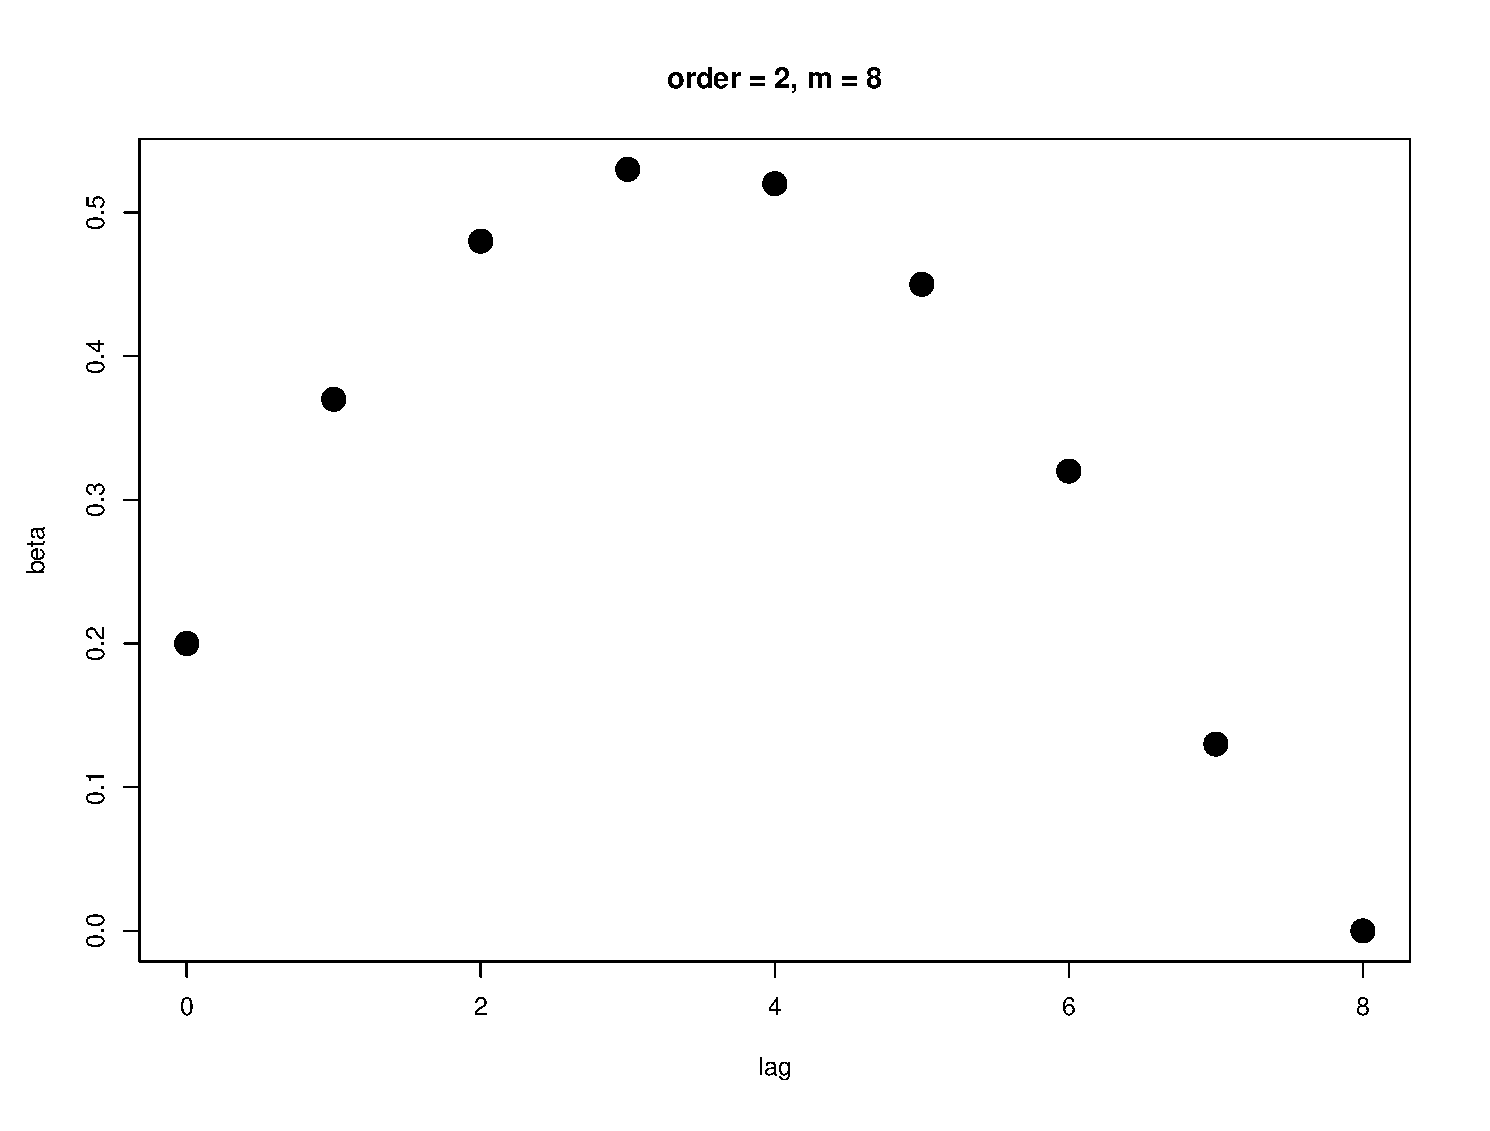
\includegraphics[width=\textwidth]{img/Polynom_2.eps}
\end{minipage}
\end{figure}
\end{frame}
%------------------------------------------------
\begin{frame}{Polynomial distributed lag}
\begin{itemize}
\item Almon-type transformation of \eqref{Almon1} for $m=8$ and $k=2$:
\begin{align} \nonumber
y_t & =  \alpha + k_0 x_t + (k_0 + k_1 + k_2)x_{t-1} + (k_0 + 2k_1 + 4k_2)x_{t-2} + \\ & + \dots + (k_0 + 8k_1 + 64k_2)x_{t-8}+u_t 
\\ \nonumber
y_t & = \alpha + k_0 (x_t + x_{t-1} + \dots + x_{t-8}) + \\ \nonumber & +  k_1(x_{t-1} + 2 x_{t-2} + \dots + 8 x_{t-8}) + \\ \nonumber & + k_2(x_{t-1} + 4x_{t-2} + \dots + 64x_{t-8}) = \\ 
y_t & = \alpha + k_0 \underbrace{\sum_{i=0}^8 x_{t-i}}_{W_{0t}} + k_1 \underbrace{\sum_{i=1}^8 i\, x_{t-i}}_{W_{1t}}  + k_2 \underbrace{\sum_{i=1}^8 i^2 x_{t-i}}_{W_{2t}}  + u_t\\
y_t & = \alpha + k_0 W_{0t} + k_1 W_{1t} + k_2 W_{2t} + u_t \label{eqpol3}
\end{align}
We estimate \eqref{eqpol3}, then calculate $\beta_i$ (lags 0 to 8) as in \eqref{eqpol2}\\
\dots note the reduction in estimated parameters (10 vs 4).
\end{itemize}
\end{frame}
%------------------------------------------------
\begin{frame}{Polynomial distributed lag}
\begin{itemize}
\item Method developed by Shirley Almon in the 60ies.
\item Equation \eqref{eqpol3} can be generalized: for $m$ lags, sums go to $m$, for higher order polynomials, we add more $W$-terms.
\vspace{0.3cm}
\item Advantages of this approach:
\begin{itemize}
\item Saves degrees of freedom
 \item Removes the problem of multicollinearity
 \item Does not affect the assumptions for $u$, because errors do not change during transformation
\end{itemize}
\vspace{0.3cm}
\item In EViews, transformation is slightly modified.
\item In R, routines are available.
\end{itemize}
\end{frame}
%------------------------------------------------
\subsection{Geometric distributed lag (Koyck) }
\begin{frame}{Geometric distributed lag (Koyck) }
IDL linear regression model: $y_t = f(x_t, x_{t-1}, x_{t-2}, \dots)$: 
\\ \vspace{0.3cm}
$ y_t = \alpha + \delta_0 x_t + \delta_1 x_{t-1} + \delta_2 x_{t-2} + \delta_3 x_{t-3} 
+ \dots + u_t$ \\ \vspace{0.3cm}
Assumption for the geometric $\delta_j$ weights:
\begin{itemize}
\item $ \delta_{j} = \gamma \rho^{\,j}$, \hspace{0.3cm} $0 < \rho < 1 $, $\hspace{0.3cm} j=0,1,2,\dots $\\
\smallskip
~~~~$\left( j \textnormal{~is the lag operator here} \right)$\\
~~~~$\delta_0 \equiv \gamma$ for convenience of notation (see RDL)\\
~~~~$|\rho|<1$ not used here (allows sign oscilations in $ \delta_{j}$).\\
\smallskip
$\delta_j = \delta_{j-1}\, \rho, \hspace{0.3cm} 0 < \rho < 1 $.\\
~~~~alternative notation of the above 
\end{itemize}
\vspace{0.3cm}
Instantaneous propensity (multiplier): $ \delta_0 = \gamma \rho^0 = \gamma$ 
\\ \vspace{0.3cm}
Long-run propensity (multiplier):
\\ \vspace{0.3cm}
$\delta_0+\delta_1+\dots=\gamma(1+\rho+\rho^2+\rho^3+\dots)=\frac{\gamma}{1-\rho}$
\end{frame}
%------------------------------------------------
\begin{frame}{Geometric distributed lag (Koyck) }
\textbf{Koyck transformation of the IDL model:}
\begin{align} 
y_t & = \alpha + \delta_0 x_t  + \delta_1 x_{t-1} \,\,+ \delta_2 x_{t-2} + \dots + u_t \hspace{0.3cm} |\delta_j = \gamma \rho^j  \notag \\
y_t & = \alpha + \gamma x_t \,\,+ \gamma\rho x_{t-1} \,+ \gamma\rho^2 x_{t-2}+\dots + u_t  \label{IDL} \\ \hline \notag \\ 
y_{t-1} & = \alpha + \gamma x_{t-1} + \gamma\rho x_{t-2} + \gamma\rho^2 x_{t-3} + \dots+u_{t-1} \hspace{0.3cm} |\times \rho 
\\ \label{eqk3}
\rho y_{t-1} & = \alpha\rho + \gamma\rho x_{t-1} + \gamma \rho^2 x_{t-2} + \dots + \rho u_{t-1}
\end{align}
\centering Now, we subtract \eqref{eqk3} from \eqref{IDL}: \par
\begin{align}
y_t-\rho y_{t-1} & = \underbrace{\alpha(1-\rho)}_{\alpha_{0}}+\gamma x_t + \underbrace{u_t-\rho u_{t-1}}_{v_t}\\
y_t & = \alpha_0 + \gamma x_t + \rho y_{t-1} + v_t \label{Koyck}
\end{align}
\end{frame}
%------------------------------------------------
\begin{frame}{Geometric distributed lag (Koyck) }
IDL model: $\quad \,y_t = \alpha + \delta_0 x_t  + \delta_1 x_{t-1} + \delta_2 x_{t-2} + \dots + u_t $\\
\medskip
Koyck transf.: $y_t = \alpha_0 + \gamma x_t + \rho y_{t-1} + v_t$ \\
\medskip
Using the Koyck transformation, we can calculate parameters \\of the IDL model from the estimated model after Koyck transformation:\\
\medskip
$\quad \hat{\delta}_0 = \hat{\gamma}$ \\
\medskip
$\quad \hat{\delta}_j = \hat{\gamma} \, \hat{\rho}^{\,j} \,\, ; \,\, j = 1,2,3, \dots$ \\
\medskip
$\quad \hat{\alpha} = \frac{\hat{\alpha}_0}{1-\hat{\rho}}$\\
\medskip
Problems of the Koyck transformation:
\begin{itemize}
    \item in \eqref{Koyck}, regressor $y_{t-1}$ is not exogenous ($v_t=u_t-\rho u_{t-1}$)\\ \dots IVR discussed separately
    \item $v_t=u_t-\rho u_{t-1}$ is not i.i.d.
    \item Koyck transformation extends to models with multiple regressors only if common $\rho$ (geometric decay) can be assumed.
\end{itemize}
\end{frame}
%------------------------------------------------
\subsection{Rational distributed lag (RDL)}
\begin{frame}{Rational distributed lag (RDL)}
The geometric distributed lag is a special case of \\rational distributed lag (RDL) model:
\begin{align} \nonumber
y_t & = \alpha_0+\gamma x_t + \rho y_{t-1} + v_t \hspace{0.3cm} \textnormal{(geometric distributed lag)}\\\label{eqrat1} 
y_t & = \alpha_0+\gamma_0 x_t +\gamma_1 x_{t-1} + \rho y_{t-1} + v_t  \hspace{0.3cm} \textnormal{ (RDL)}
\end{align}
This can be shown by successive substitution for the $y_{t-1}$ term \\of RDL equation \eqref{eqrat1}, where we get:
\begin{align}\nonumber
y_t & = \alpha + \gamma_0 x_t + (\rho \gamma_0 + \gamma_1) x_{t-1} + \rho (\rho \gamma_0 + \gamma_1) x_{t-2} +\\ & + \rho^2 (\rho \gamma_0 + \gamma_1) x_{t-3} + \rho^3 (\rho \gamma_0 + \gamma_1) x_{t-4}+ \dots \nonumber \\  &+\rho^{h-1}(\rho \gamma_0 + \gamma_1)x_{t-h} + \dots + u_t \label{eqrat2}
\end{align}
After estimating \eqref{eqrat1}, we can calculate lag distribution for \eqref{eqrat2}
\end{frame}
%------------------------------------------------
\begin{frame}{Rational distributed lag (RDL)}
RDL specification:\\
\medskip
$\quad y_t = \alpha_0+\gamma_0 x_t +\gamma_1 x_{t-1} + \rho y_{t-1}  + v_t $\\
\medskip
can be used to calculate $\delta_h$ in the IDL model:\\
\medskip
$\quad y_t = \alpha + \delta_0 x_t  + \delta_1 x_{t-1} + \delta_2 x_{t-2} + \dots + u_t $\\
\medskip
With RDLs, impact propensity $\gamma_0 \equiv \delta_0$ can differ in sign from lagged coefficients. \\
\medskip
$\delta_h = \rho^{h-1}(\rho \gamma_0 + \gamma_1)$ corresponds to the $x_{t-h}$ variable for $h \geq 1$. \\
\smallskip
~ \dots $\delta_0$ may differ in sign from ``lags'', even if $\rho > 0$.\\
~ \dots for $\rho > 0$, $\delta_h$ doesn't change sign with growing $h \geq 1$. \\
\bigskip
Long-run propensity: $\textit{LRP} = \frac{\gamma_0 + \gamma_1}{1-\rho},$\\
\smallskip
where $|\rho| < 1$ $\> \Rightarrow$ the sign of LRP follows the sign of $(\gamma_0+\gamma_1)$. \\
\medskip
Also,  $u_t = v_t + \rho v_{t-1} + \rho^2 v_{t-2} + \cdots \> \>  MA(\infty)$
\end{frame}
%------------------------------------------------
\begin{frame}{Koyck transformation and RDL model -- summary}
IDL model specification:\\ \smallskip
$y_t = \alpha + \delta_0 x_t  + \delta_1 x_{t-1} + \delta_2 x_{t-2} + \delta_3 x_{t-3}+ \dots + u_t $\\
\bigskip
Koyck: $\qquad \,\, y_t = \alpha_0 + \gamma x_t + \rho y_{t-1} + v_t$\\
\smallskip
RDL: $\qquad \quad y_t = \alpha_0+\gamma_0 x_t +\gamma_1 x_{t-1} + \rho y_{t-1}  + v_t $\\
\bigskip
\begin{table}
\centering
\caption{Koyck vs. RDL coefficients}
\label{Tab1}
\begin{tabular}{|l|c|c|}
\hline
  & Koyck & RDL \\
  \hline 
Impact multiplier & $\delta_0=\gamma~~~$ & $\delta_0=\gamma_0$ \\
\hline
Lagged multiplier (lag $h$) & $\delta_h = \gamma \rho^h$ & $\delta_h = \rho^{h-1}(\rho \gamma_0 + \gamma_1)$ \\
\hline 
LRP & $\frac{\gamma}{1-\rho}$ & $\frac{\gamma_0 + \gamma_1}{1-\rho}$\\
\hline
\end{tabular}
\end{table} 
\end{frame}
%------------------------------------------------
\subsection{Partial adjustment model (PAM)}
\begin{frame}{Partial adjustment model}
Partial adjustment model (PAM) \\is based on two main assumptions:
\begin{enumerate}
\item LRM describes long-run behavior of $y_t^{\ast}$: the unobserved, expected/equilibrium/target/optimum value of $y_t$:
\begin{equation}
{y}_t^\ast = \alpha + \beta x_t + u_t  ~~~~~~~~  \label{eqpam1} 
\end{equation}
\item Between two time periods, $y_t$ follows the process:
\begin{equation}
y_t - y_{t-1} = \theta ( y_t^\ast-y_{t-1}), \hspace{0.5cm} 0 < \theta < 1 \label{eqpam2}
\end{equation}
Hence, the actual $\Delta y_t$ is only a fraction of the ``desirable'' change from $y_{t-1}$ to the optimum value of $y_t^\ast$.
\\ \dots in the special case of $\theta = 1$, $\Delta y_t$ leads to optimum.\\
\medskip
Note: \eqref{eqpam2} can be re-written as: $y_t= \theta {y}_t^\ast + (1-\theta)y_{t-1} $
\end{enumerate}
\end{frame}
%------------------------------------------------
\begin{frame}{Partial adjustment model (PAM)}
Parameter estimation of PAM:
\begin{equation*}
{y}_t^\ast = \alpha + \beta x_t + u_t ~~~~~~~~~~~~~~~~~~~~~~~~~ \tag{\ref{eqpam1}}
\end{equation*}
\vspace{-0.6cm}
\begin{equation*}
y_t= \theta {y}_t^\ast + (1-\theta)y_{t-1}, \hspace{0.5cm} 0 < \theta < 1 \tag{\ref{eqpam2}}
\end{equation*}
\begin{enumerate}
\item Substitute for $y_t^\ast$ in \eqref{eqpam2} from \eqref{eqpam1}:\\
\begin{equation}
\begin{aligned}
y_t &= \alpha \theta &+~ \beta \theta x_t &+~ (1-\theta) y_{t-1} &+~ \theta u_t \label{eqpam3}\\
y_t &= \beta_0^{\prime} &+~ \beta_1^{\prime} x_t &+~ \beta_2^{\prime} y_{t-1} &+~ \theta u_t
\end{aligned}
\end{equation}
\item Estimate \eqref{eqpam3} and then calculate sought parameters of the PAM in \eqref{eqpam1} and \eqref{eqpam2}:\\
\smallskip
$\hat{\theta}= 1-\hat{\beta}_2^{\prime}$\\
\smallskip
$\hat{\alpha} =\hat{\beta}_0^{\prime}/\hat{\theta}$\\
\smallskip
$\hat{\beta} =\hat{\beta}_1^{\prime}/\hat{\theta}$
\end{enumerate}
\medskip
\small{\qquad Note that $\theta u_t$ can be independent of $y_{t-1}$ and i.i.d.}
\end{frame}
%------------------------------------------------
\begin{frame}{Partial adjustment model (PAM)}
Parameter interpretation of PAM:
\begin{equation*}
\begin{aligned}
{y}_t^\ast &= \alpha + \beta x_t + u_t \\
y_t &= \theta {y}_t^\ast + (1-\theta)y_{t-1}, \hspace{0.5cm} 0 < \theta < 1 \\
\hline \\
y_t &= \alpha \theta +~ \beta \theta x_t +~ (1-\theta) y_{t-1} +~ \theta u_t \\
y_t &= \beta_0^{\prime} ~+~ \beta_1^{\prime} x_t +~ \beta_2^{\prime} y_{t-1} +~ \theta u_t
\end{aligned}
\end{equation*}
\medskip
Parameters:\\
\smallskip
\begin{itemize}
\item[$\theta~:\quad$] $\theta= (1-\beta_2^{\prime})$ is the adjustment coefficient; higher $\hat{\theta}$ indicates higher speed of adjustment towards equilibrium.\\
\smallskip
\item[$\beta_1^{\prime}:\quad$] impact multiplier (short-run marginal propensity)\\
\smallskip
\item [$\beta~:\quad$] $\beta =\beta_1^{\prime}/\theta$ is the long run multiplier.
\end{itemize}
\end{frame}
%------------------------------------------------
\subsection{Adaptive expectations hypothesis (AEH)}
\begin{frame}{Adaptive expectations hypothesis (AEH)}
Adaptive expectations hypothesis (AEH) \\ model is based on two main assumptions:
\bigskip
\begin{enumerate}
\item LRM describes behavior of $y_t$, as a function of ${x}_t^\ast$: the unobserved, 
expected/equilibrium/target/optimum value \\of $x_t$ 
(permanent income, potential output, etc.):
\begin{equation}
~~~~y_t = \alpha + \beta x_t^\ast + u_t.\label{eqare1}
\end{equation}
\item The unobserved ${x}_t^\ast$ process is defined as:
\begin{equation} \label{eqare2}
\begin{aligned}
x^\ast_t - x^\ast_{t-1} & = \phi( x_t - x_{t-1}^\ast), \hspace{0.5cm} 0 < \phi < 1\\
 &  \Downarrow \\
x_t^\ast & =  \phi x_t + (1-\phi) x^\ast_{t-1}.
\end{aligned}
\end{equation}
with $\phi=0$ for static expectations\\ and $~\phi=1$ for immediate adjustment.
\end{enumerate}
\footnotesize{Note: alternative $2^{nd}$ hypothesis: $x_t^\ast =  \phi x_{t-1} + (1-\phi) x^\ast_{t-1}. $}
\end{frame}
%------------------------------------------------
\begin{frame}{Adaptive expectations hypothesis (AEH)}
Parameter estimation of AEH model:
\begin{equation}
y_t = \alpha + \beta x_t^\ast + u_t,~~ \tag{\ref{eqare1}}
\end{equation}
\begin{equation}
~~x_t^\ast =  \phi x_t + (1-\phi) x^\ast_{t-1} \tag{\ref{eqare2}}
\end{equation}
Successive substitution for $x_t^\ast$ from \eqref{eqare2} to \eqref{eqare1}: IDL process
\begin{equation}
y_t = \alpha + \beta \phi x_{t} 
    + \beta \phi (1-\phi)x_{t-1} + \beta \phi (1 - \phi)^2 x_{t-2} + \dots + u_t \label{eqare3}
 \end{equation}
After applying Koyck transformation, we get
\begin{equation} \label{eqare4}
\begin{aligned}
y_t &= \alpha \phi &+~ \beta \phi x_{t} &+~ (1-\phi) y_{t-1} &+~ v_t \\
y_t &= \beta_0^{\prime} &+~ \beta_1^{\prime} x_{t} &+~ \beta_2^{\prime} y_{t-1} &+~ v_t
\end{aligned}
\end{equation}
Estimate \eqref{eqare4}, then calculate parameters in \eqref{eqare1} and \eqref{eqare2}.
\smallskip
$\hat{\phi}= 1-\hat{\beta}_2^{\prime}$ ~~~($\phi$ is the ``adaptive expectations coefficient'')\\
\smallskip
$\hat{\alpha} =\hat{\beta}_0^{\prime}/\hat{\phi}$\\
\smallskip
$\hat{\beta} =\hat{\beta}_1^{\prime}/\hat{\phi}$ ~~~~~($\beta_1^{\prime}$ and $\beta$ are the SR and LR propensities )\\
\smallskip
\footnotesize{\qquad Note: Problems of Koyck-transformed model estimation apply.}
\end{frame}
%------------------------------------------------
\begin{frame}{Koyck, PAM, AEH: regression of $y_t$ on $x_t$ and $y_{t-1}$}
The same underlying regression model (statistical form) is used:
\begin{itemize}
\item The Koyck transformation:\\
$y_t = \alpha_0 + \gamma x_t + \rho y_{t-1} + v_t$\\
\smallskip
\item The Partial adjustment model (PAM):\\
$y_t = \alpha \theta + \beta \theta x_t + (1-\theta) y_{t-1} + \theta u_t$\\
\smallskip
\item The Model with adaptive expectations (AEM):\\
$y_t = \alpha \phi + \beta \phi x_{t} + (1-\phi) y_{t-1} + v_t $\\

\end{itemize}
\vspace{0.3cm}
We can make three different interpretations from one estimated equation.\\
\vspace{0.3cm}
Of course, not all interpretations are always relevant, we must choose according to application and test assumptions.
\end{frame}
%------------------------------------------------
\begin{frame}{Koyck, PAM, AEH: regression of $y_t$ on $x_t$ and $y_{t-1}$}
\textbf{Example:} Model for $c_t \leftarrow f(x_t,x_{t-1},x_{t-2},\dots)$:\\
private consumption $(c_t)$ as a function of disposable income $(x_t)$.\\
Same estimated model for Koyck, PAM, AEH:
\begin{equation*}
\begin{aligned}
\hat{c}_t & = &1,038~&+ &0.404 x_t~ &+ &0.501 c_{t-1} \\
\textnormal{\textbf{Koyck:}} \,\,\, \hat{c}_t & = &\hat{\alpha}_0~&+ &\hat{\gamma} x_t~ &+ &\hat{\rho} c_{t-1} 
\end{aligned}
\end{equation*}
Koyck: IDL, geometric decay in $\delta$ parameters assumed:
\begin{itemize}
\item $\hat{\rho}=0.501$
\smallskip
\item $\hat{\alpha}_0 = 1,038 = \hat{\alpha}(1-\hat{\rho}) = \hat{\alpha}(1-0.501) 
\Rightarrow \hat{\alpha}= \frac{1,038}{0.499}=2,080$
\item $\hat{\delta}_j = \hat{\gamma} \hat{\rho}^{\,j}=0.404 \times 0.501^{\,j}$
\smallskip
\item $\textit{LRP}=\frac{\hat{\gamma}}{1-\hat{\rho}}= \frac{0.404}{0.499} \doteq 0.81 $
\smallskip
\item IDL: $\hat{c}_t = 2,080 + \underbrace{0.404}_{\hat{\gamma} \hat{\rho}^{0}} x_t + \underbrace{0.202}_{\hat{\gamma} \hat{\rho}} x_{t-1} 
+ \underbrace{0.101}_{\hat{\gamma} \hat{\rho}^{2}} x_{t-2} + \dots$
\end{itemize}
\end{frame}
%------------------------------------------------
\begin{frame}{Koyck, PAM, AEH: regression of $y_t$ on $x_t$ and $y_{t-1}$}
\textbf{Example} continued:
\begin{equation*}
\begin{aligned}
\hat{c}_t & = &1,038~&+ &0.404 x_t~ &+ &0.501 c_{t-1} \\
\textnormal{\textbf{PAM:}} \,\,\, \hat{c}_t& = &\hat{\alpha} \hat{\theta}~&+ &\hat{\beta} \hat{\theta} x_t~&+ &(1-\hat{\theta}) c_{t-1} 
\end{aligned}
\end{equation*}
\begin{itemize}
\item $(1-\hat{\theta})=0.501 \Rightarrow \hat{\theta} = 0.499$
\smallskip
\item $\hat{\alpha} \hat{\theta} = 1,038 \Rightarrow \hat{\alpha}= \frac{1,038}{0.499}=2,080$
\item $\hat{\beta} \hat{\theta} = ~ 0.404 \Rightarrow \hat{\beta}= \frac{0.404}{0.499} \doteq 0.81$
\bigskip
\item PAM: $\hat{c}_t^{\ast} = 2,080 + 0.81 x_t$\\
\smallskip
$c_t - c_{t-1} = 0.499 \cdot (c_t^{\ast}-c_{t-1})$
\bigskip
\item If $c_t$ has a prominent inertia and $\Delta c_t$ significantly follows changes in habits, we might use the PAM approach.
\end{itemize}
\end{frame}
%------------------------------------------------
\begin{frame}{Koyck, PAM, AEH: regression of $y_t$ on $x_t$ and $y_{t-1}$}
\textbf{Example} continued:
\begin{equation*}
\begin{aligned}
\hat{c}_t & = &1,038~&+ &0.404 x_t~ &+ &0.501 c_{t-1} \\
\textnormal{\textbf{AEH:}} \,\,\, \hat{c}_t& = &\hat{\alpha} \hat{\phi}~&+ &\hat{\beta} \hat{\phi} x_t~&+ &(1-\hat{\phi}) c_{t-1} 
\end{aligned}
\end{equation*}
\begin{itemize}
\item $(1-\hat{\phi})=0.501 \Rightarrow \hat{\phi} = 0.499$
\smallskip
\item $\hat{\alpha} \hat{\phi} = 1,038 \Rightarrow \hat{\alpha}= \frac{1,038}{0.499}=2,080$
\item $\hat{\beta} \hat{\phi} = ~ 0.404 \Rightarrow \hat{\beta}= \frac{0.404}{0.499} \doteq 0.81$
\bigskip
\item AEH: $\hat{c}_t = 2,080 + 0.81 x_t^{\ast}$\\
\smallskip
$~~~~~~~\,x_t^{\ast} = 0.499 x_t + 0.501 x_{t-1}^{\ast}$
\bigskip
\item If $c_t$ if formed as a function of expected (e.g. permanent) income, we might prefer AEH.
\end{itemize}
\end{frame}
%------------------------------------------------
\subsection{Rational expectations}
\begin{frame}{Rational expectations}
\begin{itemize}
\item Rational expectations
$$\mathbf{E}_{t-1}(x_t)=a_0+a_1 x_{t-1} + b_1 z_{1,t-1}+b_2 z_{2, t-2}+\dots$$
$\mathbf{E}_{t-1}(x_t)$: expected value of $x_t$ at time $t-1$\\
$z_{k,t-j}$: exogenous variables with impact on $\mathbf{E}_{t-1}(x_t)$\\
\vspace{0.3cm}
We put $x_t^\ast = \mathbf{E}_{t-1}(x_t)$ into \eqref{eqare1}: $y_t = \alpha + \beta x_t^\ast + u_t$\\
\vspace{0.3cm}
We assume that agents:
\begin{itemize}
\item know all relevant information
\item know how to use this information
\end{itemize}
\vspace{0.3cm}
Agents can make prediction errors ($v_t$), so: $$x_t=x^\ast_t+v_t $$
\end{itemize}
\end{frame}
%------------------------------------------------
\begin{frame}{Rational vs. adaptive expectations}
Under rational expectations:
\vspace{0.3cm}
\begin{itemize}
\item Expected value of  prediction errors $[v_t = x_t - x^\ast_t]$ must be zero. If they were systematically different from zero, rational agents would immediately adjust their forecasting methods accordingly.
\vspace{0.3cm}
\item $[v_t = x_t - x^\ast_t]$ prediction error must be uncorrelated with any information available when the prediction is made $(t-1)$. If not, this would imply that the forecaster has not made use of all available information.
\vspace{0.3cm}
\item These properties can be used for testing the rational expectations hypothesis in different applications \\(e.g. through ex-post simulated dynamic forecasts).
\end{itemize}
\end{frame}
%------------------------------------------------
\begin{frame}{Some economic application that use expectations}
\begin{itemize}
\item Philips curve (Expectations-augmented Phillips curve)
\item Efficient market hypothesis (EMH)
\item Consumption function - Permanent income hypothesis
\end{itemize}
\end{frame}
%------------------------------------------------
\end{document}
